\documentclass[11pt]{article}
\usepackage[T1]{fontenc}
\usepackage{lmodern}
\usepackage[margin=1.1in]{geometry}
\usepackage{amsmath,amssymb,amsthm,mathtools,thmtools}
\usepackage{microtype}
\usepackage{enumitem}
\usepackage{booktabs}
\usepackage{xcolor}
\usepackage{tikz}
\usetikzlibrary{arrows.meta,positioning,calc,fit,backgrounds,decorations.pathreplacing,shapes.geometric}
\usepackage[most]{tcolorbox}
\usepackage[colorlinks=true,linkcolor=blue!50!black,citecolor=green!40!black,urlcolor=blue!50!black]{hyperref}
\usepackage[capitalise,noabbrev]{cleveref}
\hypersetup{pdftitle={Seymour's second-neighborhood conjecture: a readable account of the proof},
 pdfauthor={Rewrite by Claude (Opus 5.5) of a preprint by OpenAI}}

% ---------------------------------------------------------------- colours
\definecolor{famL}{RGB}{31,119,180}    % left family  (P, R, R')  blue
\definecolor{famR}{RGB}{214,96,26}     % right family (Q, C, C')  orange
\definecolor{zcol}{RGB}{44,140,60}     % conflict points Z         green
\definecolor{hcol}{RGB}{140,70,160}    % opposite corners H        purple
\definecolor{boxbg}{RGB}{243,246,250}
\definecolor{ideabg}{RGB}{252,248,232}

% ---------------------------------------------------------------- theorems
\declaretheorem[numberwithin=section]{theorem}
\declaretheorem[sibling=theorem]{proposition}
\declaretheorem[sibling=theorem]{lemma}
\declaretheorem[sibling=theorem]{corollary}
\declaretheorem[sibling=theorem]{claim}
\declaretheorem[sibling=theorem,style=definition]{definition}
\declaretheorem[sibling=theorem,style=definition]{example}
\declaretheorem[sibling=theorem,style=remark]{remark}
\crefname{claim}{Claim}{Claims}
\tcolorboxenvironment{theorem}{colback=boxbg,colframe=famL!60!black,boxrule=0.5pt,arc=2pt,left=4pt,right=4pt}
\tcolorboxenvironment{proposition}{colback=boxbg,colframe=famL!60!black,boxrule=0.5pt,arc=2pt,left=4pt,right=4pt}
\newtcolorbox{idea}[1][]{colback=ideabg,colframe=ideabg!50!black,boxrule=0.4pt,arc=2pt,
  left=4pt,right=4pt,fonttitle=\bfseries\small,coltitle=black,colbacktitle=ideabg!80!black!20,title={#1}}

% ---------------------------------------------------------------- macros
\newcommand{\abs}[1]{\lvert #1\rvert}
\newcommand{\RR}{\mathbb R}
\newcommand{\Rf}{\mathcal R}
\newcommand{\Cf}{\mathcal C}
\newcommand{\Mm}{\mathcal M}
\newcommand{\Ff}{F_1}
\newcommand{\Fs}{F_2}
\newcommand{\Nout}{N^+_1}
\newcommand{\Ntwo}{N^+_2}
\newcommand{\val}{\operatorname{val}}
\newcommand{\unc}{\operatorname{unc}}
\newcommand{\Lp}{\mathcal V_L}
\newcommand{\Rp}{\mathcal V_R}
\DeclareMathOperator{\rank}{rank}
\DeclareMathOperator{\im}{im}
\newcommand{\T}{\mathsf T}
\newcommand{\cL}[1]{\textcolor{famL}{#1}}
\newcommand{\cR}[1]{\textcolor{famR}{#1}}
\newcommand{\cZ}[1]{\textcolor{zcol}{#1}}
\newcommand{\cH}[1]{\textcolor{hcol}{#1}}

\tikzset{
  vtx/.style={circle,draw,fill=white,inner sep=1.5pt,minimum size=5.5mm,font=\small},
  dot/.style={circle,fill,inner sep=1.4pt},
  arc/.style={-{Stealth[length=2.2mm]},thick},
  darc/.style={-{Stealth[length=2.2mm]},thick,dashed},
  gridpt/.style={circle,draw=black!25,fill=white,inner sep=0pt,minimum size=2.2mm},
  Lpt/.style={circle,draw=famL!70!black,fill=famL,inner sep=0pt,minimum size=3.2mm},
  Rpt/.style={rectangle,draw=famR!70!black,fill=famR,inner sep=0pt,minimum size=3.0mm},
  Zpt/.style={diamond,draw=zcol!70!black,fill=zcol,inner sep=0pt,minimum size=3.8mm},
  Hpt/.style={star,star points=5,draw=hcol!70!black,fill=hcol,inner sep=0pt,minimum size=4.2mm},
}

\title{Seymour's second-neighborhood conjecture:\\ a readable account of the proof}
\author{Rewritten by Claude (Opus 5.5) from the preprint\\
\emph{A proof of Seymour's second-neighborhood conjecture}\\ by OpenAI (September 23, 2026)}
\date{November 2026}

\begin{document}
\maketitle

\begin{abstract}
An oriented graph is a directed graph without loops and without pairs of
opposite arcs. Seymour's second-neighborhood conjecture asserts that every
finite oriented graph has a vertex with at least as many vertices at
distance exactly two as at distance exactly one. A recent preprint by
OpenAI proves this conjecture in fifteen dense pages. This document
is a rewritten, expanded version of that proof. The mathematics is the same,
but we add a roadmap, intuition before each step, worked examples,
fifteen figures, and explicit verification of every inequality. We also
give a self-contained proof of the vertex-weighted forms of the conjecture.
All statements were re-checked by hand, several were tested by computer on
random instances, and the entire proof was formalized and checked in Lean~4 (see
\cref{app:checks}).
\end{abstract}

\setcounter{tocdepth}{2}
\tableofcontents

\section{Introduction}\label{sec:intro}

\subsection{The conjecture}

An \emph{oriented graph} is a finite directed graph $D$ with no loops, no
multiple arcs, and no pair of opposite arcs: for distinct vertices $x,y$ at
most one of $x\to y$ and $y\to x$ is an arc. Equivalently, it is an
orientation of a simple undirected graph. The underlying graph need not be
connected or complete.

For a vertex $v$ we write
\[
 \Nout(v)=\{u: v\to u\},\qquad
 \Ntwo(v)=\{w:\ w\ne v,\ w\notin\Nout(v),\ \text{and } v\to u\to w \text{ for some } u\}.
\]
So $\Nout(v)$ is the set of vertices at directed distance exactly one, and
$\Ntwo(v)$ is the set of vertices at directed distance \emph{exactly} two.
A vertex counts once in $\Ntwo(v)$ however many two-step paths reach it,
and a vertex that can be reached in one step does not count in $\Ntwo(v)$
even if it can also be reached in two steps (see \cref{fig:neighborhoods}).

\begin{theorem}[Seymour's second-neighborhood conjecture]\label{thm:main}
Every nonempty finite oriented graph $D$ has a vertex $v$ with
\[
 \abs{\Nout(v)}\le\abs{\Ntwo(v)}.
\]
\end{theorem}

Following the literature, a vertex satisfying this inequality is called a
\emph{Seymour vertex}. A sink (a vertex of outdegree $0$) is trivially a
Seymour vertex, so the content of the theorem lies in graphs where every
vertex has an out-neighbor.

\begin{figure}[ht]
\centering
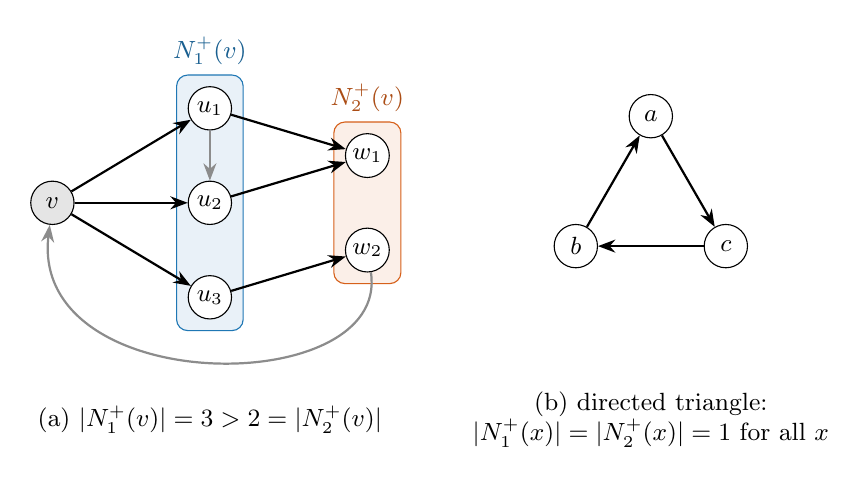
\begin{tikzpicture}[scale=1]
 \begin{scope}
 \node[vtx,fill=black!10] (v) at (0,0) {$v$};
 \node[vtx] (u1) at (2,1.2) {$u_1$};
 \node[vtx] (u2) at (2,0) {$u_2$};
 \node[vtx] (u3) at (2,-1.2) {$u_3$};
 \node[vtx] (w1) at (4,0.6) {$w_1$};
 \node[vtx] (w2) at (4,-0.6) {$w_2$};
 \foreach \u in {u1,u2,u3} \draw[arc] (v)--(\u);
 \draw[arc] (u1)--(w1); \draw[arc] (u2)--(w1); \draw[arc] (u3)--(w2);
 \draw[arc,black!45] (u1)--(u2);
 \draw[arc,black!45] (w2) .. controls (4.3,-2.5) and (-0.3,-2.5) .. (v);
 \begin{scope}[on background layer]
  \node[draw=famL,fill=famL!10,rounded corners,fit=(u1)(u3),inner sep=4pt,
        label={[famL!80!black,font=\small]above:$\Nout(v)$}] {};
  \node[draw=famR,fill=famR!10,rounded corners,fit=(w1)(w2),inner sep=4pt,
        label={[famR!80!black,font=\small]above:$\Ntwo(v)$}] {};
 \end{scope}
 \node[font=\small,align=center] at (2,-2.75) {(a) $\abs{\Nout(v)}=3>2=\abs{\Ntwo(v)}$};
 \end{scope}
 \begin{scope}[xshift=7.6cm]
 \node[vtx] (a) at (90:1.1) {$a$};
 \node[vtx] (b) at (210:1.1) {$b$};
 \node[vtx] (c) at (330:1.1) {$c$};
 \draw[arc] (a)--(c); \draw[arc] (c)--(b); \draw[arc] (b)--(a);
 \node[font=\small,align=center] at (0,-2.75) {(b) directed triangle:\\
   $\abs{\Nout(x)}=\abs{\Ntwo(x)}=1$ for all $x$};
 \end{scope}
\end{tikzpicture}
\caption{(a) The first and second out-neighborhoods of $v$. The arc
$u_1\to u_2$ does not put $u_2$ into $\Ntwo(v)$, because $u_2$ is already at
distance one. The arc $w_2\to v$ is irrelevant for $v$. In this picture $v$
is not a Seymour vertex, but $w_1$ (a sink) is. (b) In a directed
triangle every vertex is a Seymour vertex with equality, so the inequality
of \cref{thm:main} cannot be made strict.}
\label{fig:neighborhoods}
\end{figure}

\subsection{Background}

The conjecture was stated by Seymour and recorded by Dean and
Latka~\cite{DeanLatka1995}. For \emph{tournaments} (an arc between every
pair of vertices) it is Dean's conjecture, proved by
Fisher~\cite{Fisher1996} with a probability distribution obtained from
Farkas' lemma, and later combinatorially by Havet and
Thomass\'e~\cite{HavetThomasse2000} using median orders. It was extended
to tournaments missing a matching, a star or a
clique~\cite{FidlerYuster2007}, generalized stars~\cite{Ghazal2012},
a matching together with a star~\cite{DaraFrancisJacobNarayanan2022}, and
two stars~\cite{DaamouchAlMninyGhazal2025}. It is known for minimum
outdegree at most six~\cite{KanekoLocke2001} (and, by a computer-assisted
preprint, seven~\cite{SadhukhanSandeepSen2026}). In general, some vertex has
$\abs{\Ntwo(v)}\ge\gamma\abs{\Nout(v)}$ with
$\gamma\approx0.657$~\cite{ChenShenYuster2003}, improved to
$\gamma\approx0.7155$~\cite{HuangPeng2024}. Orientations of random graphs
were treated in~\cite{BotlerMouraNaia2023,EspunyDiazEtAl2025} and dense
graphs in~\cite{Brukhman2026}.
The proof below builds on two earlier ideas: the minimal counterexample and
graph-product (blow-up) method of Brantner, Brockman, Kay and
Snively~\cite{BrantnerBrockmanKaySnively2009}, and Seacrest's idea of
studying the conjecture for \emph{sets} of vertices~\cite{Seacrest2019}.

\subsection{The proof at a glance}\label{sec:glance}

The proof is by contradiction and has three stages, shown in
\cref{fig:proofmap}. Throughout, for a digraph $D$ and a set $S$ of
vertices we use the \emph{forward image}
\[
 F(S)=F_D(S)=\{y:\ x\to y \text{ for some } x\in S\},\qquad F^2(S)=F(F(S)).
\]
Note that $F(S)$ may intersect $S$. Since an oriented graph has no
directed closed walk of length two, $v\notin F^2(\{v\})$ and therefore
$\Ntwo(v)=F^2(\{v\})\setminus F(\{v\})$.

\begin{figure}[ht]
\centering
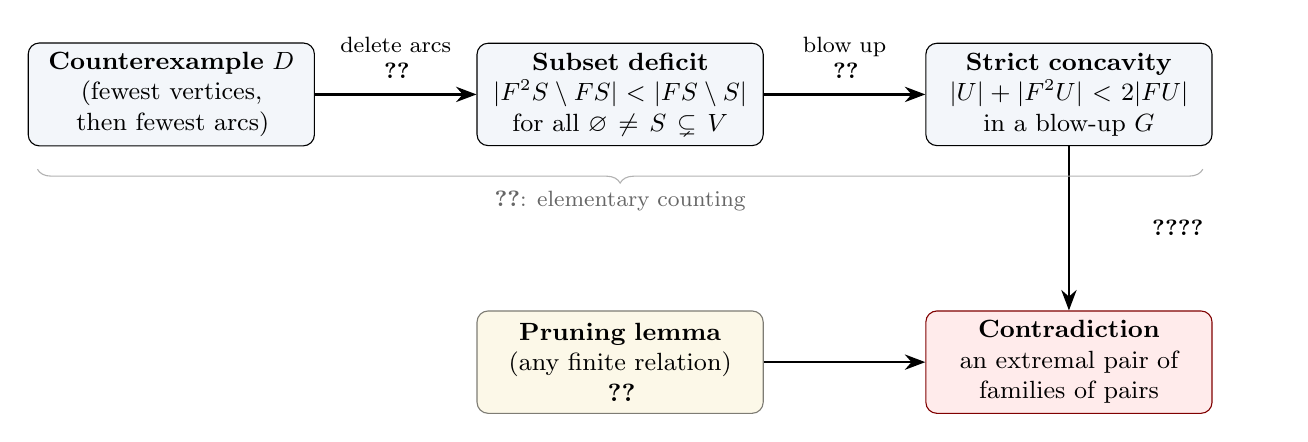
\begin{tikzpicture}[
  box/.style={draw,rounded corners,align=center,font=\small,fill=boxbg,minimum height=13mm,text width=34mm},
  key/.style={box,fill=ideabg,draw=ideabg!50!black},
  lab/.style={font=\footnotesize,align=center,text width=22mm},
  every edge/.style={draw,-{Stealth[length=2.6mm]},thick}]
 \node[box] (ce) at (0,0) {\textbf{Counterexample} $D$\\ (fewest vertices,\\ then fewest arcs)};
 \node[box] (sd) at (5.7,0) {\textbf{Subset deficit}\\ $\abs{F^2S\setminus FS}<\abs{FS\setminus S}$\\ for all $\varnothing\ne S\subsetneq V$};
 \node[box] (cc) at (11.4,0) {\textbf{Strict concavity}\\ $\abs U+\abs{F^2U}<2\abs{FU}$\\ in a blow-up $G$};
 \node[key] (pr) at (5.7,-3.4) {\textbf{Pruning lemma}\\ (any finite relation)\\ \cref{sec:pruning}};
 \node[box,fill=red!8,draw=red!50!black] (con) at (11.4,-3.4) {\textbf{Contradiction}\\ an extremal pair of\\ families of pairs};
 \draw (ce) edge node[lab,above=2pt] {delete arcs\\\cref{lem:subset-deficit}} (sd);
 \draw (sd) edge node[lab,above=2pt] {blow up\\\cref{lem:blowup}} (cc);
 \draw (cc) edge node[lab,right=1pt,text width=24mm] {\cref{sec:pairs,sec:contradiction}} (con);
 \draw (pr) edge (con);
 \node[font=\footnotesize,text=black!60] at (5.7,-1.35) {\cref{sec:reduction}: elementary counting};
 \draw[black!30,decorate,decoration={brace,amplitude=5pt,mirror}] (-1.7,-0.95)--(13.1,-0.95);
\end{tikzpicture}
\caption{Map of the proof. The top row (\cref{sec:reduction}) is a
reduction that uses only elementary counting. The genuinely new ingredient
is the pruning lemma (\cref{sec:pruning}), which holds for every finite
binary relation. \Cref{sec:contradiction} combines the two.}
\label{fig:proofmap}
\end{figure}

\paragraph{Stage 1: from one vertex to all sets (\cref{sec:reduction}).}
Take a counterexample $D$ with the fewest vertices and, among those, the
fewest arcs. Deleting arcs creates a smaller graph, which must therefore
have a Seymour vertex; analysing what that vertex lost shows that every
nonempty proper set $S$ of vertices of $D$ satisfies the \emph{subset
deficit}
\[
 \abs{F^2(S)\setminus F(S)}<\abs{F(S)\setminus S}.
\]
In words: the second step from $S$ reaches fewer new vertices (outside
$F(S)$) than the first step reaches outside $S$. It is \emph{not} a comparison
of $\abs{F^2(S)}$ with $\abs{F(S)}$: the part $S\cap F(S)$ of the first image
does not count. The gap between the two is the error term
$\abs{S\setminus F(S)}$ of \cref{rem:error-term}.

\paragraph{Stage 2: a cleaner inequality (\cref{sec:reduction}).}
The subset deficit is awkward to sum over many sets because of the error
term $\abs{S\setminus F(S)}$ explained in \cref{rem:error-term}. Replacing
every vertex by a large transitive tournament drowns this error term and
produces an oriented graph $G$ in which all indegrees are positive and every
nonempty proper set $U$ is \emph{strictly concave}:
\[
 \abs{U}+\abs{F^2(U)}<2\abs{F(U)}.
\]
This says the sequence $\abs U,\abs{F(U)},\abs{F^2(U)}$ is strictly concave:
the second increment is smaller than the first.

\paragraph{Stage 3: no graph is strictly concave
(\cref{sec:pairs,sec:pruning,sec:contradiction}).}
This is the heart of the proof. We work with \emph{sets of ordered pairs}
of vertices, drawn as subsets of a grid $X\times X$. On pairs there are two
natural image operators: $\Ff$ moves the first coordinate along an arc and
$\Fs$ moves the second. We consider pairs $(P,Q)$ of such families that are
\emph{compatible} ($\Ff P$ and $\Fs Q$ are disjoint), both containing the
diagonal, and we pick one maximizing
\[
 \val(P,Q)=\abs P+\abs Q+\#\{\text{grid points covered by neither }\Ff P\text{ nor }\Fs Q\}.
\]
Strict concavity, applied to every column of $P$ and every row of $Q$,
produces new families that are larger by a definite amount. They may fail to
be compatible, but the \emph{pruning lemma} restores compatibility at a cost
that is paid exactly by the gain. The new pair has a larger value, a
contradiction.

\begin{idea}[Where is the novelty?]
Stages~1 and~2 adapt known techniques (Seacrest's arc-deletion argument and
the blow-up of Brantner et al.) and are elementary. The new idea is
Stage~3 and, in particular, the pruning lemma. It is a statement about an
arbitrary finite relation and has nothing to do with orientations. Its proof
bounds the size of a matching in an auxiliary bipartite graph by linear
algebra: a single ``conflict matrix'' is factored in two different ways, and
a generic choice of coefficients turns the combinatorics into rank
inequalities. The key feature of the lemma is that its cost depends on the
points that are left \emph{uncovered after} pruning; this is what makes
the accounting in Stage~3 close up.
\end{idea}

\subsection{Conventions}

All graphs and sets are finite. $\abs{S}$ is the size of $S$. For an
integer-valued quantity, a strict inequality $a<b$ is often used in the form
$a\le b-1$. The table below lists the main notation. It mostly agrees with
the original preprint, and \cref{app:dictionary} lists the few changes.

\begin{center}
\small
\begin{tabular}{@{}lll@{}}
\toprule
Symbol & Meaning & Introduced in\\
\midrule
$\Nout(v),\ \Ntwo(v)$ & vertices at distance exactly one, exactly two & \cref{sec:intro}\\
$F(S),\ F^2(S)$ & forward image of a vertex set, and its iterate & \cref{sec:glance}\\
$I,\ E,\ T,\ Q,\ C$ & sets in the arc-deletion argument & \cref{sec:subset-deficit}\\
$G=D[T_m]$ & blow-up by transitive tournaments & \cref{sec:blowup}\\
$X\times X$, $\Delta$ & grid of ordered pairs, its diagonal & \cref{sec:pairs}\\
$\Ff,\ \Fs$ & move first / second coordinate along an arc & \cref{def:coord-images}\\
$P_j,\ Q_i$ & column $j$ of $P$, row $i$ of $Q$ & \cref{def:coord-images}\\
\cL{$P,\ \Rf,\ P'$} / \cR{$Q,\ \Cf,\ Q'$} & left / right families (blue / orange in figures) & \cref{sec:pairs}\\
conflict, compatible & $\Ff\{r\}\cap\Fs\{c\}\ne\varnothing$; no conflicts & \cref{def:conflict}\\
$\unc(P,Q)$, $\val(P,Q)$ & number of uncovered points; $\abs P+\abs Q+\unc(P,Q)$ & \cref{def:value}\\
\cZ{$Z$} / \cH{$H$} & conflict points / opposite corners (green / purple) & \cref{def:ZH}\\
$\Gamma$, $\Mm$ & augmented bipartite graph, a maximum matching & \cref{sec:gamma}\\
$L,N,A,B$ & four coefficient matrices with $NL=AB$ & \cref{sec:matrices}\\
\bottomrule
\end{tabular}
\end{center}

\section{From a counterexample to strict concavity}\label{sec:reduction}

\begin{idea}[What this section does]
We assume \cref{thm:main} fails and produce an oriented graph $G$ with
positive indegrees in which every nonempty proper vertex set $U$ satisfies
$\abs U+\abs{F^2U}<2\abs{FU}$ (\cref{prop:reduction}). This takes two steps.
First, a minimal counterexample satisfies a ``subset'' version of the
conjecture's failure (\cref{lem:subset-deficit}). Second, a blow-up turns
that subset version into the clean concavity inequality
(\cref{lem:blowup}). Only elementary counting is used.
\end{idea}

Throughout this section $F=F_D$ is the forward image in a fixed digraph $D$
(defined in \cref{sec:glance}); it is \emph{not} required that $F(S)$ be
disjoint from $S$.

\subsection{Minimal counterexamples}

Call an oriented graph $D$ a \emph{counterexample} if it is nonempty and
$\abs{\Nout(v)}>\abs{\Ntwo(v)}$ for every vertex $v$. A counterexample is
\emph{minimal} if it has the minimum number of vertices among all
counterexamples and, subject to this, the minimum number of arcs.

\begin{lemma}\label{lem:strong}
A minimal counterexample $D$ is strongly connected, has at least two
vertices, and every vertex has an in-neighbor.
\end{lemma}

\begin{proof}
A sink $v$ would satisfy $\abs{\Nout(v)}=0\le\abs{\Ntwo(v)}$, so $D$ has no
sink; in particular $D$ has at least two vertices. Suppose $D$ is not
strongly connected. Then some strongly connected component $K$ has no arc
leaving it (a ``sink component'' of the condensation), and $K\ne V(D)$.
For $v\in K$, all vertices reachable from $v$ lie in $K$, so $\Nout(v)$ and
$\Ntwo(v)$ are the same in $D$ and in the induced subgraph $D[K]$. Hence $D[K]$
is a counterexample with fewer vertices, which is impossible. So $D$ is
strongly connected. Since $D$ has at least two vertices, every vertex then
has an in-neighbor.
\end{proof}

\subsection{The subset deficit}\label{sec:subset-deficit}

The defining property of a counterexample concerns single vertices. The
next lemma upgrades it to all nonempty proper sets, at the price of
replacing $\Nout$ and $\Ntwo$ by the set analogues $F(S)\setminus S$ and
$F^2(S)\setminus F(S)$. For $S=\{v\}$ these are exactly $\Nout(v)$ and
$\Ntwo(v)$, so the lemma generalizes the counterexample property.

\begin{lemma}[Subset deficit]\label{lem:subset-deficit}
Let $D$ be a minimal counterexample. Then
\begin{equation}\label{eq:subset-deficit}
 \abs{F^2(S)\setminus F(S)}<\abs{F(S)\setminus S}
 \qquad\text{for every }\varnothing\ne S\subsetneq V(D).
\end{equation}
\end{lemma}

The argument adapts the proof of~\cite[Lemma~4]{Seacrest2019}, where the
right-hand side is $\abs{F(S)}$. Here we need the stronger right-hand side
$\abs{F(S)\setminus S}$, and this is why we minimize the number of vertices
before the number of arcs (to get strong connectivity).

\paragraph{Intuition.}
Fix $S$. Split $F(S)$ into the part $I=F(S)\cap S$ inside $S$ and the part
$E=F(S)\setminus S$ outside. Since $F(I)\subseteq F(S)$, everything in
$F^2(S)\setminus F(S)$ is reached from $E$. We ``switch on'' the vertices
of $E$ in batches. Each time a batch $Q$ is switched on, the set of vertices
reached from the switched-on part grows, and we show that it grows by
fewer than $\abs Q$ vertices. The batch $Q$ comes from a Seymour vertex
$v\in S$ of a graph with fewer arcs, and the growth is bounded by comparing
what $v$ has in $D$ with what it has in the smaller graph.

\begin{figure}[ht]
\centering
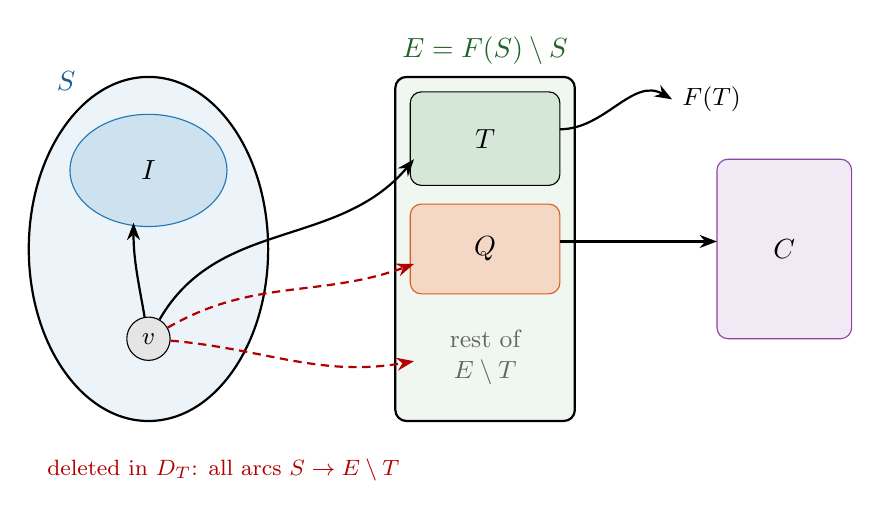
\begin{tikzpicture}[scale=0.95]
 % S
 \draw[thick,fill=famL!8] (0,0) ellipse (1.6 and 2.3);
 \node[famL!80!black] at (-1.1,2.25) {$S$};
 \draw[fill=famL!22,draw=famL] (0,1.05) ellipse (1.05 and 0.75);
 \node at (0,1.05) {$I$};
 \node[vtx,fill=black!10] (v) at (0,-1.2) {$v$};
 % E
 \draw[thick,rounded corners,fill=zcol!7] (3.3,-2.3) rectangle (5.7,2.3);
 \node[zcol!70!black] at (4.5,2.65) {$E=F(S)\setminus S$};
 \draw[rounded corners,fill=zcol!20] (3.5,0.85) rectangle (5.5,2.1);
 \node at (4.5,1.47) {$T$};
 \draw[rounded corners,fill=famR!25,draw=famR] (3.5,-0.6) rectangle (5.5,0.6);
 \node at (4.5,0) {$Q$};
 \node[font=\small,align=center,text=black!60] at (4.5,-1.45) {rest of\\ $E\setminus T$};
 % C
 \draw[rounded corners,fill=hcol!12,draw=hcol] (7.6,-1.2) rectangle (9.4,1.2);
 \node[align=center] at (8.5,0) {$C$};
 % arcs
 \draw[arc,red!70!black,densely dashed] (v) to[out=30,in=200] (3.55,-0.2);
 \draw[arc,red!70!black,densely dashed] (v) to[out=-5,in=190] (3.55,-1.5);
 \draw[arc] (v) to[out=60,in=230] (3.55,1.2);
 \draw[arc] (v) to[out=100,in=-90] (-0.2,0.35);
 \draw[arc] (5.5,0.1) -- (7.6,0.1);
 \draw[arc] (5.5,1.6) to[out=0,in=150] (7.0,2.0) node[right,font=\small] {$F(T)$};
 \node[font=\footnotesize,red!70!black,align=center] at (1.0,-2.95) {deleted in $D_T$: all arcs $S\to E\setminus T$};
\end{tikzpicture}
\caption{One step in the proof of \cref{lem:subset-deficit}, with
$I=F(S)\cap S$. All arcs from
$S$ to $E\setminus T$ are deleted (dashed). The minimal choice of $D$ gives a
Seymour vertex $v$ of the smaller graph $D_T$. It must lie in $S$ and lose
its out-neighbors $Q\subseteq E\setminus T$. The set $C$ consists of vertices
that $v$ reached in two steps only through $Q$. Since $v$ is not a Seymour
vertex of $D$, $\abs C-\abs{Q\cap F(T)}<\abs Q$.}
\label{fig:deletion}
\end{figure}

\begin{proof}[Proof of \cref{lem:subset-deficit}]
Fix $\varnothing\ne S\subsetneq V(D)$ and set
\[
 I=F(S)\cap S,\qquad E=F(S)\setminus S,\qquad
 g(T)=\abs{F(T)\setminus(I\cup T)}\quad\text{for }T\subseteq E.
\]
Since $D$ is strongly connected (\cref{lem:strong}) and $S$ is a nonempty
proper subset, some arc leaves $S$; hence $E\ne\varnothing$. Also
$g(\varnothing)=0$.

\emph{Step 1: the target is $g(E)$.} Since $F(S)=I\cup E$ and
$F(I)\subseteq F(S)$ (because $I\subseteq S$),
\[
 F^2(S)\setminus F(S)=\bigl(F(I)\cup F(E)\bigr)\setminus(I\cup E)
 =F(E)\setminus(I\cup E),
\]
so $\abs{F^2(S)\setminus F(S)}=g(E)$, and we must show $g(E)<\abs E$.

\emph{Step 2: one batch.} We claim that for every $T\subsetneq E$ there is a
nonempty $Q\subseteq E\setminus T$ with
\begin{equation}\label{eq:increment}
 g(T\cup Q)-g(T)<\abs Q.
\end{equation}
Let $D_T$ be obtained from $D$ by deleting all arcs from $S$ to $E\setminus T$
(\cref{fig:deletion}). Every vertex of $E\setminus T\neq\varnothing$ has an
in-neighbor in $S$, so at least one arc is deleted. $D_T$ has the same
vertices and fewer arcs than $D$, so by minimality it is not a
counterexample: some vertex $v$ satisfies
$\abs{N^+_{1,D_T}(v)}\le\abs{N^+_{2,D_T}(v)}$.

\begin{itemize}[leftmargin=*]
\item \emph{$v$ lost an out-neighbor.} Otherwise $N^+_{1,D_T}(v)=\Nout(v)$, and
since deleting arcs can only shrink $F^2(\{v\})$, also
$N^+_{2,D_T}(v)\subseteq\Ntwo(v)$. Then $v$ would be a Seymour vertex of $D$.
Hence $v\in S$ and
\[
 Q:=\Nout(v)\cap(E\setminus T)\ne\varnothing
\]
is exactly the set of out-neighbors that $v$ lost. As
$\Nout(v)\subseteq F(S)=I\cup E$, we get $\Nout(v)\subseteq I\cup T\cup Q$
and $N^+_{1,D_T}(v)=\Nout(v)\setminus Q\subseteq I\cup T$.

\item \emph{Where $v$ can go in two steps in $D_T$.} A path $v\to u\to w$ in
$D_T$ has $u\in I\cup T$. If $u\in I\subseteq S$, then $w\in F(S)$ but $w\notin
E\setminus T$ (those arcs were deleted), so $w\in I\cup T$. If $u\in T$,
then $w\in F(T)$. Thus
\begin{equation}\label{eq:DT-reach}
 F^2_{D_T}(\{v\})\subseteq I\cup T\cup F(T).
\end{equation}

\item \emph{Gains.} A vertex $w\in N^+_{2,D_T}(v)\setminus\Ntwo(v)$ is reached
in two steps in $D_T$, hence in $D$, and $w\ne v$; so the only way it was
not in $\Ntwo(v)$ is that $w\in\Nout(v)$. As $w\notin N^+_{1,D_T}(v)$, we get
$w\in Q$, and by~\eqref{eq:DT-reach} and $Q\cap(I\cup T)=\varnothing$,
$w\in Q\cap F(T)$. So at most $\abs{Q\cap F(T)}$ vertices are gained.

\item \emph{Losses.} Put $C=F(Q)\setminus(I\cup T\cup Q\cup F(T))$. Every
$c\in C$ is reached from $v$ via some $q\in Q$. It is not an out-neighbor of
$v$, because $\Nout(v)\subseteq I\cup T\cup Q$. And $c\ne v$, since an arc
$q\to v$ would be opposite to $v\to q$ (\emph{here orientation is used}).
So $C\subseteq\Ntwo(v)$. By~\eqref{eq:DT-reach}, no vertex of $C$ is in
$F^2_{D_T}(\{v\})$. So all of $C$ is lost.
\end{itemize}
Writing $d_1=\abs{\Nout(v)}$ and $d_2=\abs{\Ntwo(v)}$, the Seymour property of
$v$ in $D_T$ and the gains/losses give
\[
 d_1-\abs Q=\abs{N^+_{1,D_T}(v)}\le\abs{N^+_{2,D_T}(v)}\le d_2-\abs C+\abs{Q\cap F(T)}.
\]
On the other hand, the increment of $g$ is exactly
\begin{equation}\label{eq:g-increment}
 g(T\cup Q)-g(T)=\abs C-\abs{Q\cap F(T)}.
\end{equation}
Indeed $F(T\cup Q)\setminus(I\cup T\cup Q)$ is the disjoint union of
$F(T)\setminus(I\cup T\cup Q)$ and $C$, and the first set is
$F(T)\setminus(I\cup T)$ with the points of $Q\cap F(T)$ removed (recall
$Q\cap(I\cup T)=\varnothing$). Combining, and using $d_2<d_1$ because $D$ is a
counterexample,
\[
 g(T\cup Q)-g(T)=\abs C-\abs{Q\cap F(T)}\le\abs Q+d_2-d_1<\abs Q,
\]
which is~\eqref{eq:increment}.

\emph{Step 3: summing.} Start from $T_0=\varnothing$ and, as long as
$T_k\ne E$, apply Step~2 (always to the \emph{original} $D$) to get
$Q_k$ and set $T_{k+1}=T_k\cup Q_k$. The sets $Q_k$ are nonempty and
disjoint, so the process ends with $T_K=E$ after $K\ge1$ steps (as
$E\neq\varnothing$). Summing~\eqref{eq:increment},
\[
 g(E)=g(\varnothing)+\sum_{k<K}\bigl(g(T_{k+1})-g(T_k)\bigr)<\sum_{k<K}\abs{Q_k}=\abs E.
\]
By Step~1 this is~\eqref{eq:subset-deficit}.
\end{proof}

\subsection{Why the deficit is not yet enough}

The subset deficit has a nice form, but we will need to \emph{add} the
inequality over many sets, and for that the following cleaner quantity is
better suited:
\[
 \kappa(S)=\abs S-2\abs{F(S)}+\abs{F^2(S)}
 =\bigl(\abs{F^2S}-\abs{FS}\bigr)-\bigl(\abs{FS}-\abs S\bigr),
\]
the ``second difference'' of the sequence $\abs S,\abs{FS},\abs{F^2S}$. It is
a plain combination of cardinalities with no set differences, so it adds
up well (we will use this in \cref{eq:fiber-sum}).

\begin{remark}[The error term]\label{rem:error-term}
For every digraph and every set $S$,
\begin{equation}\label{eq:error-term}
 \kappa(S)\le\bigl(\abs{F^2S\setminus FS}-\abs{FS\setminus S}\bigr)+\abs{S\setminus FS}.
\end{equation}
Indeed, $\abs{F^2S}-\abs{FS}\le\abs{F^2S\setminus FS}$ and
$\abs{FS}-\abs S=\abs{FS\setminus S}-\abs{S\setminus FS}$. So the subset deficit
gives $\kappa(S)\le -1+\abs{S\setminus F(S)}$, which is useless when many
vertices of $S$ receive no arc from $S$. The blow-up below multiplies the
bracket in~\eqref{eq:error-term} by a large factor $m$ while increasing the
error term by at most one per vertex of $D$.
\end{remark}

\subsection{Blowing up by transitive tournaments}\label{sec:blowup}

Let $T_m$ be the \emph{transitive tournament} on $\{1,\dots,m\}$, with
$a\to b$ if and only if $a<b$. We write $f$ for its forward image.

\begin{lemma}[Internal estimate]\label{lem:internal}
For every nonempty $T\subseteq\{1,\dots,m\}$,
\[
 \abs T-2\abs{f(T)}+\abs{f^2(T)}\le 1 .
\]
\end{lemma}

\begin{proof}
Let $a=\min T$. Then $f(T)=\{a+1,\dots,m\}$ and $f^2(T)=\{a+2,\dots,m\}$,
while $\abs T\le m-a+1$. If $a<m$ the left side is at most
$(m-a+1)-2(m-a)+(m-a-1)=0$. If $a=m$ then $T=\{m\}$ and the left side is
$1-0+0=1$.
\end{proof}

For example, in $T_5$ the set $T=\{2,4\}$ has $f(T)=\{3,4,5\}$ and
$f^2(T)=\{4,5\}$, giving $2-6+2=-2\le1$. The point of the transitive
tournament is that a nonempty set loses at most one element under $f$
($\abs{f(T)}\ge\abs T-1$). If we blew up by independent sets instead, a block
would have empty image and the error would be as large as $m$.

\begin{definition}[Blow-up]
Let $D$ be an oriented graph and $m\ge1$. The \emph{blow-up} $G=D[T_m]$ has
vertex set $V(D)\times\{1,\dots,m\}$. Its arcs are
\[
 (v,a)\to(w,b)\iff v\to w\text{ in }D,\ \text{or}\ v=w\text{ and }a<b.
\]
The set $\{v\}\times\{1,\dots,m\}$ is the \emph{block} of $v$. Arcs inside a
block are \emph{internal} and arcs between blocks are \emph{external}.
\end{definition}

\begin{figure}[ht]
\centering
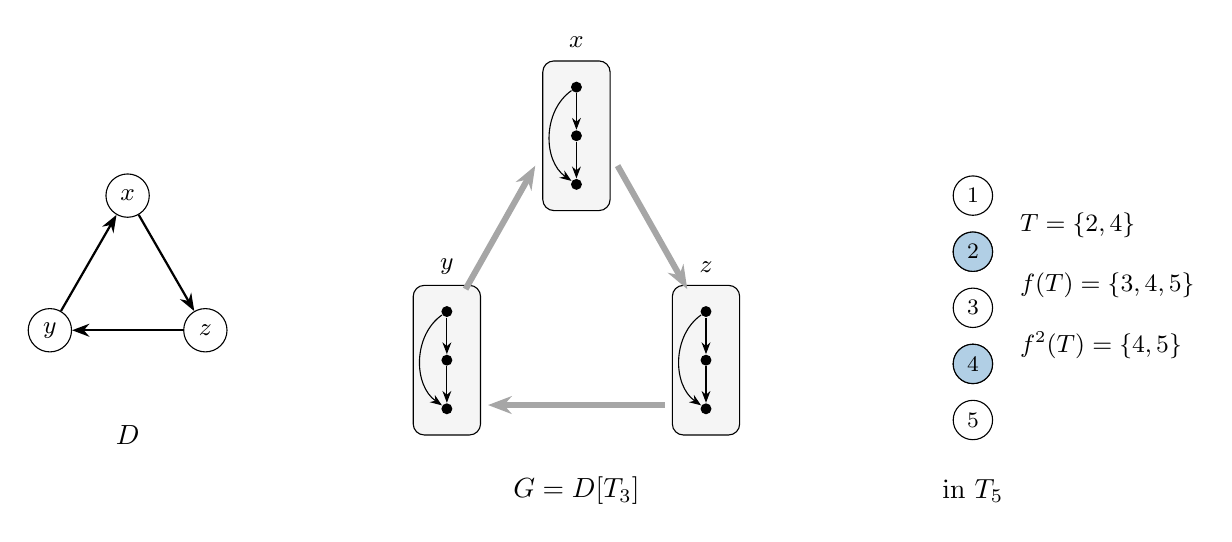
\begin{tikzpicture}[scale=0.95]
 \begin{scope}
  \node[vtx] (a) at (90:1.2) {$x$};
  \node[vtx] (b) at (210:1.2) {$y$};
  \node[vtx] (c) at (330:1.2) {$z$};
  \draw[arc] (a)--(c); \draw[arc] (c)--(b); \draw[arc] (b)--(a);
  \node at (0,-2.0) {$D$};
 \end{scope}
 \begin{scope}[xshift=6.0cm]
  \foreach \nm/\ang in {x/90,y/210,z/330}{
   \begin{scope}[shift={(\ang:2.0)}]
    \draw[rounded corners,fill=black!4] (-0.45,-1.0) rectangle (0.45,1.0);
    \node[dot] (\nm1) at (0,0.65) {}; \node[dot] (\nm2) at (0,0) {}; \node[dot] (\nm3) at (0,-0.65) {};
    \draw[-{Stealth[length=1.5mm]}] (\nm1)--(\nm2);
    \draw[-{Stealth[length=1.5mm]}] (\nm2)--(\nm3);
    \draw[-{Stealth[length=1.5mm]}] (\nm1) to[bend right=55] (\nm3);
    \node[font=\small] at (0,1.25) {$\nm$};
   \end{scope}}
  \draw[-{Stealth[length=3mm]},line width=2.2pt,black!35] (90:2.0)++(0.55,-0.4) -- ($(330:2.0)+(-0.25,0.95)$);
  \draw[-{Stealth[length=3mm]},line width=2.2pt,black!35] ($(330:2.0)+(-0.55,-0.6)$) -- ($(210:2.0)+(0.55,-0.6)$);
  \draw[-{Stealth[length=3mm]},line width=2.2pt,black!35] ($(210:2.0)+(0.25,0.95)$) -- ($(90:2.0)+(-0.55,-0.4)$);
  \node at (0,-2.75) {$G=D[T_3]$};
 \end{scope}
 \begin{scope}[xshift=11.3cm,yshift=1.2cm]
  \foreach \k in {1,...,5} \node[vtx,minimum size=5mm,font=\footnotesize] (t\k) at (0,-0.75*\k+0.75) {\k};
  \foreach \k in {2,4} \node[vtx,minimum size=5mm,font=\footnotesize,fill=famL!35] at (t\k) {\k};
  \node[font=\small,align=left,anchor=west] at (0.5,-0.4) {$T=\{2,4\}$};
  \node[font=\small,align=left,anchor=west] at (0.5,-1.2) {$f(T)=\{3,4,5\}$};
  \node[font=\small,align=left,anchor=west] at (0.5,-2.0) {$f^2(T)=\{4,5\}$};
  \node at (0,-3.95) {in $T_5$};
 \end{scope}
\end{tikzpicture}
\caption{Left: a base graph $D$ (a directed triangle). Middle: its blow-up
$D[T_3]$. Each vertex becomes a transitive tournament, and each arc becomes
all $9$ arcs between the corresponding blocks (thick grey arrows). Right:
images inside a transitive tournament (vertices ordered top to bottom; every
arc points downwards).}
\label{fig:blowup}
\end{figure}

\begin{lemma}[Blow-up]\label{lem:blowup}
Let $D$ be an oriented graph on $n\ge1$ vertices in which every vertex has
an in-neighbor and which satisfies~\eqref{eq:subset-deficit}. Let $m>n$ and
$G=D[T_m]$. Then $G$ is an oriented graph, every vertex of $G$ has an
in-neighbor, and
\begin{equation}\label{eq:strict-concavity}
 \abs U+\abs{F_G^2(U)}<2\abs{F_G(U)}\qquad\text{for every }\varnothing\ne U\subsetneq V(G).
\end{equation}
\end{lemma}

The same blow-up appears in~\cite[Theorem~4.3]{BrantnerBrockmanKaySnively2009},
where it is applied to single vertices. Here we need the estimate for all
sets.

\begin{proof}
$G$ is oriented: internal arcs go from smaller to larger labels, and two
opposite external arcs would come from opposite arcs of $D$. Each $(w,b)$
receives an arc from the block of an in-neighbor of $w$ in $D$.

Fix $\varnothing\ne U\subsetneq V(G)$. For $v\in V(D)$ let
$T_v=\{a:(v,a)\in U\}$ and let $S=\{v:T_v\ne\varnothing\}$ be the
\emph{support} of $U$. We compute block by block.

\emph{First image (exact).} An external arc into the block of $w$ starting
in $U$ exists only if $w\in F(S)$, and then it reaches \emph{every} vertex of
the block. Internal arcs from $U$ into the block of $w$ reach exactly
$\{w\}\times f(T_w)$. Hence the block of $w$ meets $F_G(U)$ in the whole block
if $w\in F(S)$, in $\{w\}\times f(T_w)$ if $w\in S\setminus F(S)$, and not at all
otherwise:
\begin{equation}\label{eq:first-image}
 \abs{F_G(U)}=m\abs{F(S)}+\sum_{w\in S\setminus F(S)}\abs{f(T_w)}.
\end{equation}

\emph{Second image (upper bound).} Consider a path of length two starting in
$U$. If both arcs are external, it ends in a block of $F^2(S)$. If exactly
one is external, it ends in a block of $F(S)$. If the internal step comes
first, the path stays in a block of $S$ and then moves to a block of $F(S)$.
If the external step comes first, it moves to a block of $F(S)$ and the
internal step stays in that block. If
both arcs are internal, it stays in the block of some $v\in S$ and ends in
$\{v\}\times f^2(T_v)$. Writing $H_0=F(S)\cup F^2(S)$, and counting the blocks
of $H_0$ in full, we get
\begin{equation}\label{eq:second-image}
 \abs{F_G^2(U)}\le m\abs{H_0}+\sum_{v\in S\setminus H_0}\abs{f^2(T_v)}
 \le m\abs{H_0}+\sum_{v\in S\setminus F(S)}\abs{f^2(T_v)},
\end{equation}
where the last step only adds nonnegative terms (as $F(S)\subseteq H_0$).

\emph{Combining.} Split $\abs U=\sum_{v\in S\cap F(S)}\abs{T_v}+\sum_{v\in S\setminus F(S)}\abs{T_v}$.
From~\eqref{eq:first-image} and~\eqref{eq:second-image},
\[
 \abs U-2\abs{F_GU}+\abs{F_G^2U}
 \le m\abs{H_0}-2m\abs{F(S)}+\sum_{v\in S\cap F(S)}\abs{T_v}
 +\sum_{v\in S\setminus F(S)}\Bigl(\abs{T_v}-2\abs{f(T_v)}+\abs{f^2(T_v)}\Bigr).
\]
Use $\abs{T_v}\le m$ in the first sum and \cref{lem:internal} in the second:
\[
 \abs U-2\abs{F_GU}+\abs{F_G^2U}\le m\bigl(\abs{H_0}-2\abs{F(S)}+\abs{S\cap F(S)}\bigr)+\abs{S\setminus F(S)}.
\]
Since $\abs{H_0}=\abs{F(S)}+\abs{F^2(S)\setminus F(S)}$ and
$\abs{F(S)}-\abs{S\cap F(S)}=\abs{F(S)\setminus S}$, the bracket equals
$\abs{F^2(S)\setminus F(S)}-\abs{F(S)\setminus S}$. We have shown, for every
$U$,
\begin{equation}\label{eq:blowup-master}
 \abs U-2\abs{F_GU}+\abs{F_G^2U}\le m\bigl(\abs{F^2S\setminus FS}-\abs{FS\setminus S}\bigr)+\abs{S\setminus FS},
\end{equation}
which is the scaled version of~\eqref{eq:error-term} announced in
\cref{rem:error-term}.

\emph{Case $S\ne V(D)$.} By~\eqref{eq:subset-deficit} the bracket is an integer
$\le-1$, and $\abs{S\setminus F(S)}\le n$, so the right side is at most
$-m+n<0$.

\emph{Case $S=V(D)$.} Every vertex of $D$ has an in-neighbor, so
$F(S)=V(D)$ and every block is filled: $F_G(U)=V(G)$. Since every vertex of
$G$ has an in-neighbor, $F_G^2(U)=F_G(V(G))=V(G)$ too. Thus the left side
equals $\abs U-\abs{V(G)}<0$, as $U$ is proper.
\end{proof}

\begin{proposition}[Counterexample reduction]\label{prop:reduction}
If \cref{thm:main} fails, there is a nonempty oriented graph $G$ in which
every vertex has an in-neighbor and~\eqref{eq:strict-concavity} holds for
every nonempty proper vertex set $U$.
\end{proposition}

\begin{proof}
Take a minimal counterexample $D$. By \cref{lem:strong,lem:subset-deficit}
it has positive indegrees and satisfies~\eqref{eq:subset-deficit}. Apply
\cref{lem:blowup} with any $m>\abs{V(D)}$.
\end{proof}

\begin{idea}[What we have achieved, and what is used later]
From now on we only use the graph $G$ and two of its properties:
\textbf{(G1)} $G$ is a nonempty oriented graph in which every vertex has an
in-neighbor; \textbf{(G2)} every nonempty proper $U\subseteq V(G)$ is
strictly concave, $\abs U+\abs{F^2U}<2\abs{FU}$. The remaining sections show
that (G1) and (G2) are incompatible.
\end{idea}

\section{Pairs of vertices: the grid picture}\label{sec:pairs}

\begin{idea}[What this section does]
We introduce the language of the rest of the proof: subsets of the grid
$X\times X$, the two coordinate images $\Ff,\Fs$, conflicts and compatibility,
and the quantity $\val(P,Q)$ that will be maximized. We then explain
\emph{heuristically} why maximizing $\val$ leads to a contradiction. The
explanation is made rigorous in \cref{sec:contradiction}, and the one
missing tool, the pruning lemma, is proved in \cref{sec:pruning}.
\end{idea}

\subsection{Coordinate images}

In this section and the next, $X$ is a finite set with an arbitrary binary
relation $\to$. Loops $x\to x$ and pairs of opposite arrows are
allowed; this generality is needed for the pruning lemma. In
\cref{sec:contradiction} the relation will be the arc relation of the graph
$G$ from \cref{prop:reduction}. We write $F(U)=\{y: x\to y\text{ for some }x\in U\}$
as before.

\emph{Drawing convention.} A pair $(i,j)\in X\times X$ is drawn in
\textbf{row $i$ and column $j$} of a square grid. So the first coordinate is
vertical and the second is horizontal.

\begin{definition}[Coordinate images, columns, rows]\label{def:coord-images}
For $S\subseteq X\times X$ let
\begin{align*}
 \Ff S&=\{(i,j):\ (p,j)\in S\text{ and }p\to i\text{ for some }p\}
 &&\text{(move the first coordinate),}\\
 \Fs S&=\{(i,j):\ (i,s)\in S\text{ and }s\to j\text{ for some }s\}
 &&\text{(move the second coordinate),}
\end{align*}
and $\Ff^2=\Ff\circ\Ff$, $\Fs^2=\Fs\circ\Fs$. The \emph{column} $j$ of $P$ and the
\emph{row} $i$ of $Q$ are
\[
 P_j=\{p:(p,j)\in P\},\qquad Q_i=\{s:(i,s)\in Q\}.
\]
\end{definition}

So $\Ff$ moves points \emph{vertically} inside their column and $\Fs$ moves
points \emph{horizontally} inside their row (\cref{fig:coord}). Each
operator acts on the lines of the grid independently, by the ordinary
image $F$:
\begin{equation}\label{eq:columnwise}
 (\Ff P)_j=F(P_j),\quad (\Ff^2P)_j=F^2(P_j),\qquad
 (\Fs Q)_i=F(Q_i),\quad (\Fs^2Q)_i=F^2(Q_i).
\end{equation}
In particular $\abs{\Ff P}=\sum_j\abs{F(P_j)}$ and $\abs{\Fs Q}=\sum_i\abs{F(Q_i)}$.
This is how an inequality about vertex sets, such as strict concavity,
becomes an inequality about sets of pairs: apply it to every column (or
row) and add.

\begin{figure}[ht]
\centering
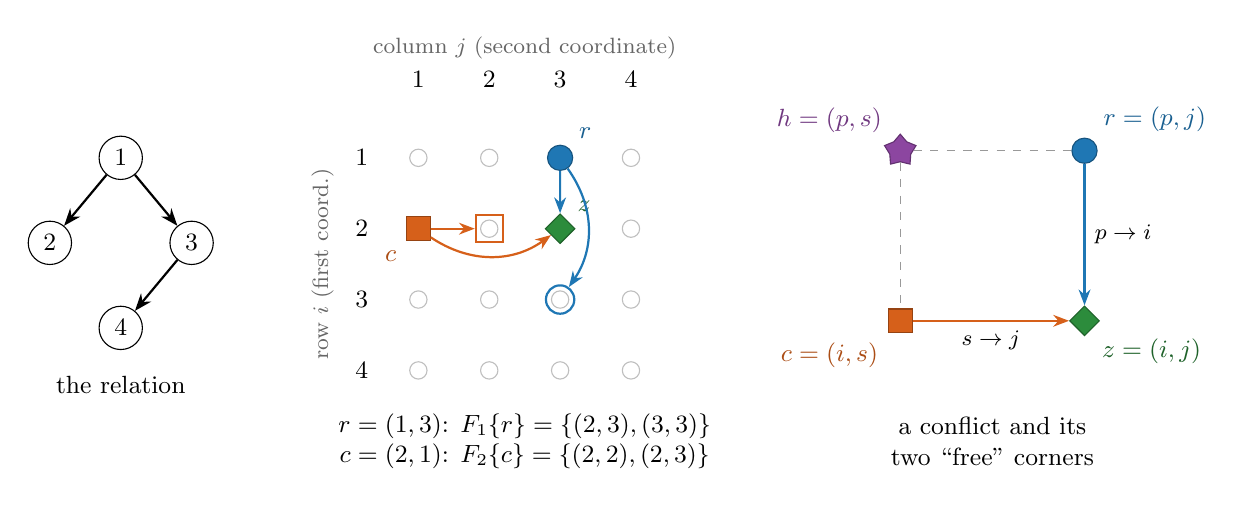
\begin{tikzpicture}[scale=0.9]
 % relation
 \begin{scope}[xshift=-3.2cm,yshift=-2.2cm]
  \node[vtx] (n1) at (0,1.2) {$1$};
  \node[vtx] (n2) at (-1,0) {$2$};
  \node[vtx] (n3) at (1,0) {$3$};
  \node[vtx] (n4) at (0,-1.2) {$4$};
  \draw[arc] (n1)--(n2); \draw[arc] (n1)--(n3); \draw[arc] (n3)--(n4);
  \node[font=\small] at (0,-2.0) {the relation};
 \end{scope}
 % grid
 \begin{scope}
  \foreach \k in {1,...,4} {
   \node[font=\small] at (\k,0.1) {$\k$};
   \node[font=\small] at (0.2,-\k) {$\k$};
  }
  \node[font=\footnotesize,text=black!60] at (2.5,0.55) {column $j$ (second coordinate)};
  \node[font=\footnotesize,text=black!60,rotate=90] at (-0.35,-2.5) {row $i$ (first coord.)};
  \foreach \i in {1,...,4} \foreach \j in {1,...,4} \node[gridpt] at (\j,-\i) {};
  \node[Lpt,label={[famL!80!black,font=\small]above right:$r$}] (r) at (3,-1) {};
  \node[Rpt,label={[famR!80!black,font=\small]below left:$c$}] (c) at (1,-2) {};
  \node[Zpt,label={[zcol!70!black,font=\small]above right:$z$}] (z) at (3,-2) {};
  \node[circle,draw=famL,thick,inner sep=0pt,minimum size=3.6mm] (r3) at (3,-3) {};
  \node[rectangle,draw=famR,thick,inner sep=0pt,minimum size=3.4mm] (c2) at (2,-2) {};
  \draw[-{Stealth[length=2mm]},famL,thick] (r) -- (z);
  \draw[-{Stealth[length=2mm]},famL,thick] (r) to[bend left=35] (r3);
  \draw[-{Stealth[length=2mm]},famR,thick] (c) -- (c2);
  \draw[-{Stealth[length=2mm]},famR,thick] (c) to[bend right=35] (z);
  \node[font=\small,align=center] at (2.5,-5.0) {$r=(1,3)$: $\Ff\{r\}=\{(2,3),(3,3)\}$\\
   $c=(2,1)$: $\Fs\{c\}=\{(2,2),(2,3)\}$};
 \end{scope}
 % abstract rectangle
 \begin{scope}[xshift=7.8cm,yshift=-0.9cm]
  \node[Hpt,label={[hcol!80!black,font=\small]above left:$h=(p,s)$}] (h) at (0,0) {};
  \node[Lpt,label={[famL!80!black,font=\small]above right:$r=(p,j)$}] (rr) at (2.6,0) {};
  \node[Rpt,label={[famR!80!black,font=\small]below left:$c=(i,s)$}] (cc) at (0,-2.4) {};
  \node[Zpt,label={[zcol!70!black,font=\small]below right:$z=(i,j)$}] (zz) at (2.6,-2.4) {};
  \draw[-{Stealth[length=2mm]},thick,famL] (rr) -- node[right,font=\footnotesize,black] {$p\to i$} (zz);
  \draw[-{Stealth[length=2mm]},thick,famR] (cc) -- node[below,font=\footnotesize,black] {$s\to j$} (zz);
  \draw[black!40,dashed] (h)--(rr); \draw[black!40,dashed] (h)--(cc);
  \node[font=\small,align=center] at (1.3,-4.1) {a conflict and its\\ two ``free'' corners};
 \end{scope}
\end{tikzpicture}
\caption{Left: a relation on $X=\{1,2,3,4\}$. Middle: the grid $X\times X$
(row $=$ first coordinate). The blue point $r$ moves vertically under $\Ff$,
the orange point $c$ moves horizontally under $\Fs$, and their images meet
at the green point $z$. So $r$ and $c$ \emph{conflict}. Right: in general a
conflict between $r=(p,j)$ and $c=(i,s)$ spans a rectangle. The meeting
point $z=(i,j)$ is the opposite corner to the purple point $h=(p,s)$.}
\label{fig:coord}
\end{figure}

\subsection{Conflicts and compatibility}

Throughout, we deal with a \emph{left} family (drawn blue: $P$, $\Rf$, $P'$),
to which $\Ff$ is applied, and a \emph{right} family (drawn orange: $Q$,
$\Cf$, $Q'$), to which $\Fs$ is applied.

\begin{definition}[Conflict, compatibility]\label{def:conflict}
A left member $r=(p,j)$ and a right member $c=(i,s)$ \emph{conflict} if
\[
 p\to i\qquad\text{and}\qquad s\to j.
\]
A left family $P$ and a right family $Q$ are \emph{compatible} if no member
of $P$ conflicts with a member of $Q$.
\end{definition}

\begin{lemma}\label{lem:conflict-geometry}
\begin{enumerate}[label=(\alph*)]
\item $r=(p,j)$ and $c=(i,s)$ conflict if and only if $\Ff\{r\}\cap\Fs\{c\}\ne\varnothing$,
and then $\Ff\{r\}\cap\Fs\{c\}=\{(i,j)\}$.
\item $P$ and $Q$ are compatible if and only if $\Ff P\cap\Fs Q=\varnothing$.
\end{enumerate}
\end{lemma}

\begin{proof}
(a) $\Ff\{r\}$ lies in column $j$ and $\Fs\{c\}$ lies in row $i$, so they can
only meet at $(i,j)$. This point is in $\Ff\{r\}$ if and only if $p\to i$, and
in $\Fs\{c\}$ if and only if $s\to j$. (b) follows from (a), since
$\Ff P=\bigcup_{r\in P}\Ff\{r\}$ and $\Fs Q=\bigcup_{c\in Q}\Fs\{c\}$.
\end{proof}

We say that a left member $r$ \emph{covers} the points of $\Ff\{r\}$, and a
right member $c$ covers the points of $\Fs\{c\}$. So the points covered by a
pair of families $(P,Q)$ are those of $\Ff P\cup\Fs Q$.

\begin{definition}[Conflict points and opposite corners]\label{def:ZH}
For a left family $\Rf$ and a right family $\Cf$ let
\begin{align*}
 \cZ{Z}&=\{(i,j):\ (p,j)\in\Rf\text{ conflicts with }(i,s)\in\Cf\text{ for some }p,s\},\\
 \cH{H}&=\{(p,s):\ (p,j)\in\Rf\text{ conflicts with }(i,s)\in\Cf\text{ for some }i,j\}.
\end{align*}
\end{definition}

So every conflict spans a rectangle with corners $r,z,c,h$ as in
\cref{fig:coord}. The conflict point $z$ is the point both members cover,
and $h$ is the remaining corner. Conversely, $z$ and $h$ determine the
conflict: $r=(h_1,z_2)$ and $c=(z_1,h_2)$.

\subsection{The extremal set-up}

Now let the relation be the arc relation of a nonempty oriented graph $G$
with vertex set $X$, and let $\Delta=\{(v,v):v\in X\}$ be the diagonal.

\begin{definition}[Uncovered points, value, admissible pairs]\label{def:value}
For compatible families $P,Q\subseteq X\times X$ put
\[
 \unc(P,Q)=\abs X^2-\abs{\Ff P}-\abs{\Fs Q},\qquad
 \val(P,Q)=\abs P+\abs Q+\unc(P,Q).
\]
By \cref{lem:conflict-geometry}(b), $\unc(P,Q)$ is the number of grid points
covered by \emph{neither} family. A pair $(P,Q)$ is \emph{admissible} if it
is compatible and $\Delta\subseteq P\cap Q$.
\end{definition}

\begin{lemma}\label{lem:diag-compatible}
$(\Delta,\Delta)$ is admissible. In particular admissible pairs exist, and since
there are finitely many, some admissible pair maximizes $\val$.
\end{lemma}

\begin{proof}
A point $(i,j)\in\Ff\Delta\cap\Fs\Delta$ would require $j\to i$ (from
$(j,j)\in\Delta$) and $i\to j$ (from $(i,i)\in\Delta$). These are opposite
arcs, which an oriented graph does not have.
\end{proof}

\subsection{Why maximizing the value leads to a contradiction}\label{sec:ledger}

Here is the plan of \cref{sec:contradiction}, with the verifications
postponed. Let $(P,Q)$ be an admissible pair of maximum value, write
$\mu=\abs P+\abs Q$ and $d=\unc(P,Q)$, so $\val(P,Q)=\mu+d$.

\begin{enumerate}[label=\textbf{\arabic*.},leftmargin=*]
\item \textbf{Concavity on every line.} Every column $P_j$ and every row $Q_i$ is a
nonempty proper subset of $X$. Applying strict concavity to each and adding
(using~\eqref{eq:columnwise}) gives
\[
 \abs P+\abs{\Ff^2P}<2\abs{\Ff P},\qquad \abs Q+\abs{\Fs^2Q}<2\abs{\Fs Q}.
\]
\item \textbf{Complement.} Let $\Rf=(X\times X)\setminus\Fs^2Q$ and $\Cf=(X\times X)\setminus\Ff^2P$.
Adding the two inequalities shows $\abs\Rf+\abs\Cf>\mu+2d$. This is a gain of
more than $d$ over the old value.
\item \textbf{Repair.} $(\Rf,\Cf)$ contains the diagonal but may have conflicts. The
pruning lemma deletes some members to remove all conflicts. The number
deleted is at most $\abs H$ plus the number of points of $Z$ left
uncovered. We will see that $\abs H\le d$, and the uncovered points number
at most $d'$, the value of $\unc$ for the new pair.
\item \textbf{New value.} The new pair $(P',Q')$ is admissible and
\[
 \val(P',Q')\ \ge\ (\abs\Rf+\abs\Cf)-(d+d')+d'\ >\ \mu+2d-d=\mu+d=\val(P,Q),
\]
contradicting maximality.
\end{enumerate}

\begin{figure}[ht]
\centering
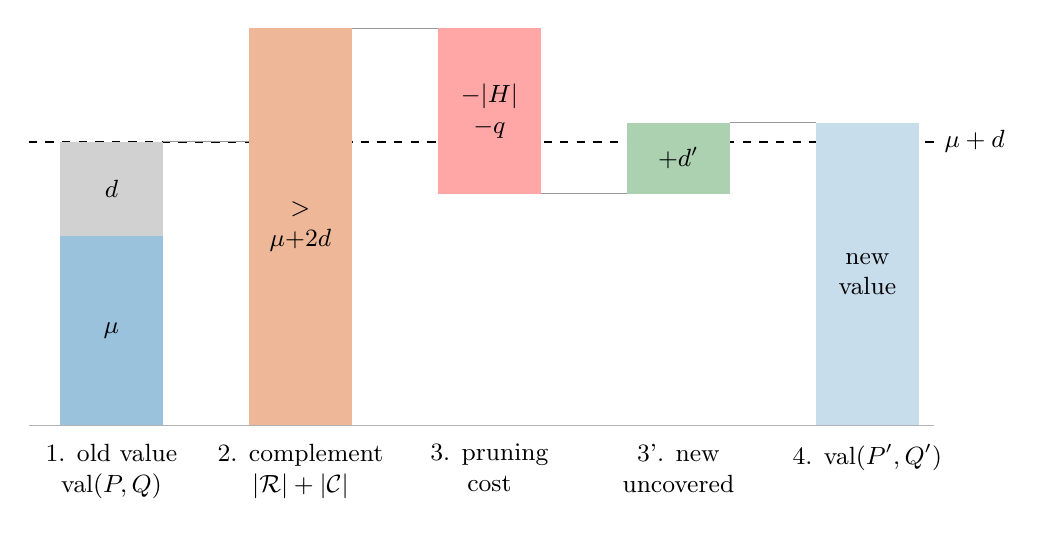
\begin{tikzpicture}[yscale=0.6,xscale=1.0,lab/.style={font=\small,align=center,anchor=north}]
 \def\bw{1.3}
 % levels: mu=4, d=2, d'=1.5 ; R+C = 8.4
 \draw[black!30] (-0.4,0)--(11.1,0);
 \draw[dashed,thick] (-0.4,6)--(11.1,6) node[right,font=\small] {$\mu+d$};
 \fill[famL!45] (0,0) rectangle (\bw,4); \fill[black!18] (0,4) rectangle (\bw,6);
 \node[font=\small] at (0.65,2) {$\mu$}; \node[font=\small] at (0.65,5) {$d$};
 \node[lab] at (0.65,-0.2) {1. old value\\$\val(P,Q)$};
 \fill[famR!45] (2.4,0) rectangle (2.4+\bw,8.4);
 \node[font=\small,align=center] at (3.05,4.2) {$>$\\$\mu{+}2d$};
 \node[lab] at (3.05,-0.2) {2. complement\\$\abs\Rf+\abs\Cf$};
 \fill[red!35] (4.8,4.9) rectangle (4.8+\bw,8.4);
 \node[font=\small,align=center] at (5.45,6.65) {$-\abs H$\\$-q$};
 \node[lab] at (5.45,-0.2) {3. pruning\\cost};
 \fill[zcol!40] (7.2,4.9) rectangle (7.2+\bw,6.4);
 \node[font=\small] at (7.85,5.65) {$+d'$};
 \node[lab] at (7.85,-0.2) {3'. new\\uncovered};
 \fill[famL!25] (9.6,0) rectangle (9.6+\bw,6.4);
 \node[font=\small,align=center] at (10.25,3.2) {new\\value};
 \node[lab] at (10.25,-0.2) {4. $\val(P',Q')$};
 \draw[black!40] (\bw,6)--(2.4,6); \draw[black!40] (2.4+\bw,8.4)--(4.8,8.4);
 \draw[black!40] (4.8+\bw,4.9)--(7.2,4.9); \draw[black!40] (7.2+\bw,6.4)--(9.6,6.4);
\end{tikzpicture}
\caption{The ledger: steps 1--4 above as bar heights. Here $q\le d'$ is the
number of conflict points left uncovered after pruning, so the loss
$\abs H+q\le d+d'$ is more than paid for by the gain and the returned $d'$.
The new bar ends above the dashed line.}
\label{fig:ledger}
\end{figure}

\begin{remark}[Why this particular value]\label{rem:why-value}
If we maximized only $\abs P+\abs Q$, the ledger would give a new size
$>\mu+d-d'$, which need not exceed $\mu$. If we used $\abs P+\abs Q+\lambda\,\unc$
for some $\lambda>0$, the ledger would give $\val_\lambda(P',Q')>\mu+d+(\lambda-1)d'$
against the old value $\mu+\lambda d$. The new value is at least the old one
exactly when $\mu+d+(\lambda-1)d'\ge\mu+\lambda d$, that is, when
$(\lambda-1)(d'-d)\ge0$. Since $d'-d$ can have either sign, this holds for
every $d,d'\ge0$ only when $\lambda=1$. (The strict increase comes from the
strict inequality in the ledger, not from the weight.) So it is essential that the pruning cost is charged partly
to points left uncovered \emph{after} pruning ($d'$), and that this charge
enters with the same weight as the uncovered points in the value.
\end{remark}

\section{The pruning lemma}\label{sec:pruning}

\begin{idea}[What this section does]
Given a left family $\Rf$ and a right family $\Cf$ that may conflict, we
delete some members so that no conflicts remain. The pruning lemma bounds
the number of deletions by $\abs H$ plus the number of conflict points that
end up uncovered. The proof has two parts.
(1)~A purely combinatorial reduction: it suffices to show that a certain
bipartite graph $\Gamma$ has no matching larger than $\abs Z+\abs H$
(\cref{sec:gamma}).
(2)~A linear-algebra proof of this matching bound
(\cref{sec:strategy,sec:matrices,sec:rank,sec:generic,sec:kernel}).
Nothing in this section uses orientation. The relation $\to$ on $X$ is
arbitrary.
\end{idea}

\subsection{Statement and examples}

Recall from \cref{sec:pairs} that a left member $r$ covers $\Ff\{r\}$, a right
member $c$ covers $\Fs\{c\}$, and $Z$ and $H$ are the conflict points and
opposite corners of the conflicts between $\Rf$ and $\Cf$
(\cref{def:ZH}).

\begin{lemma}[Pruning lemma; Lemma~3.1 of the original]\label{lem:pruning}
Let $X$ be a finite set with an arbitrary relation $\to$, and let
$\Rf,\Cf\subseteq X\times X$. There are $\Rf'\subseteq\Rf$ and $\Cf'\subseteq\Cf$ such that
\begin{enumerate}[label=\textup{(P\arabic*)}]
\item\label{P1} $\Rf'$ and $\Cf'$ are compatible;
\item\label{P2} every member of $\Rf\cup\Cf$ that conflicts with no member of the
other family is kept;
\item\label{P3} the number of deleted members satisfies
\begin{equation}\label{eq:pruning-bound}
 \abs{\Rf\setminus\Rf'}+\abs{\Cf\setminus\Cf'}\ \le\ \abs H+\bigl\lvert Z\setminus(\Ff\Rf'\cup\Fs\Cf')\bigr\rvert .
\end{equation}
\end{enumerate}
\end{lemma}

The last term counts the conflict points that no kept member covers. The
two families are always counted separately, even when a pair belongs to both.

\begin{example}[One conflict]\label{ex:one-conflict}
If $\Rf=\{r\}$ and $\Cf=\{c\}$ conflict, then $Z=\{z\}$ and $H=\{h\}$ as in
\cref{fig:coord}. Deleting $r$ costs $1\le\abs H$.
\end{example}

\begin{example}[Deleting more can be cheaper]\label{ex:K22}
Let $X=\{0,1,2,3\}$ with the four arrows $0\to1$, $0\to2$, $3\to1$, $3\to2$, and
\[
 \Rf=\{(0,1),(0,2)\},\qquad \Cf=\{(1,3),(2,3)\}
\]
(\cref{fig:K22grid}). A left member $(0,j)$ and a right member $(i,3)$
conflict because $0\to i$ and $3\to j$. So all four pairs conflict, and
\[
 Z=\{1,2\}\times\{1,2\},\qquad H=\{(0,3)\}.
\]
Compatible subfamilies must have $\Rf'=\varnothing$ or $\Cf'=\varnothing$.
Deleting one whole family costs $2$, but then every point of $Z$ is still
covered by the other family: $(i,3)$ covers $(i,1),(i,2)$. So the right side
of~\eqref{eq:pruning-bound} is only $\abs H=1$. The bound fails for the
\emph{cheapest} pruning! It holds for deleting three members ($3\le1+2$) or
all four ($4\le1+4$). The construction in the proof deletes all four.
\end{example}

\begin{figure}[ht]
\centering
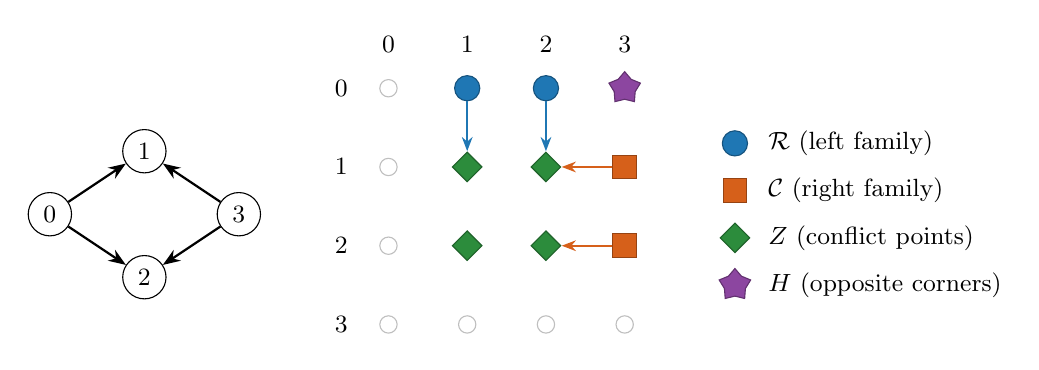
\begin{tikzpicture}[scale=1.0]
 \begin{scope}
  \node[vtx] (x0) at (0,0) {$0$};
  \node[vtx] (x1) at (1.2,0.8) {$1$};
  \node[vtx] (x2) at (1.2,-0.8) {$2$};
  \node[vtx] (x3) at (2.4,0) {$3$};
  \draw[arc] (x0)--(x1); \draw[arc] (x0)--(x2);
  \draw[arc] (x3)--(x1); \draw[arc] (x3)--(x2);
 \end{scope}
 \begin{scope}[xshift=4.3cm,yshift=1.6cm]
  \foreach \k in {0,1,2,3} {\node[font=\small] at (\k,0.55) {$\k$}; \node[font=\small] at (-0.6,-\k) {$\k$};}
  \foreach \i in {0,1,2,3} \foreach \j in {0,1,2,3} \node[gridpt] at (\j,-\i) {};
  \foreach \i in {1,2} \foreach \j in {1,2} \node[Zpt] at (\j,-\i) {};
  \node[Hpt] at (3,0) {};
  \node[Lpt] (r1) at (1,0) {}; \node[Lpt] (r2) at (2,0) {};
  \node[Rpt] (c1) at (3,-1) {}; \node[Rpt] (c2) at (3,-2) {};
  \draw[famL,-{Stealth[length=1.8mm]},thick] (r1)--(1,-0.8);
  \draw[famL,-{Stealth[length=1.8mm]},thick] (r2)--(2,-0.8);
  \draw[famR,-{Stealth[length=1.8mm]},thick] (c1)--(2.2,-1);
  \draw[famR,-{Stealth[length=1.8mm]},thick] (c2)--(2.2,-2);
 \end{scope}
 \begin{scope}[xshift=8.7cm,yshift=0.9cm,font=\small]
  \node[Lpt] at (0,0) {}; \node[anchor=west] at (0.3,0) {$\Rf$ (left family)};
  \node[Rpt] at (0,-0.6) {}; \node[anchor=west] at (0.3,-0.6) {$\Cf$ (right family)};
  \node[Zpt] at (0,-1.2) {}; \node[anchor=west] at (0.3,-1.2) {$Z$ (conflict points)};
  \node[Hpt] at (0,-1.8) {}; \node[anchor=west] at (0.3,-1.8) {$H$ (opposite corners)};
 \end{scope}
\end{tikzpicture}
\caption{\Cref{ex:K22}. The left members (blue, row $0$) cover the green
points below them. The right members (orange, column $3$) cover the green
points to their left. Each of the four conflicts has the same opposite
corner $(0,3)$. Removing all conflicts cheaply is impossible relative to
$\abs H=1$. The lemma pays for the deletions with the green points that are
left uncovered.}
\label{fig:K22grid}
\end{figure}

\Cref{ex:K22} shows that \ref{P3} is \emph{not} an upper bound on the
minimum number of deletions. It is an exchange rate. Every deletion beyond
$\abs H$ must be paid for by a conflict point that becomes uncovered. In the
application (\cref{sec:contradiction}) uncovered points count in the
objective exactly like members, so such trades are free.

\begin{example}[Deleting less is necessary]\label{ex:star}
The opposite extreme. Let
$X=\{p_1,\dots,p_n\}\sqcup\{j_1,\dots,j_n\}\sqcup\{i_0,s_0\}$ with the
arrows $p_k\to i_0$ and $s_0\to j_m$ for all $k,m$, and
\[
 \Rf=\{(p_k,j_m):1\le k,m\le n\},\qquad\Cf=\{c\},\quad c=(i_0,s_0).
\]
Every $(p_k,j_m)$ conflicts with $c$, because $p_k\to i_0$ and $s_0\to j_m$
(\cref{fig:star}). So all $n^2+1$ members are in conflicts, while
\[
 Z=\{(i_0,j_m):m\le n\},\qquad H=\{(p_k,s_0):k\le n\},\qquad \abs Z+\abs H=2n.
\]
Deleting every member that is in a conflict costs $n^2+1$, far above the
budget $\abs H+\abs Z=2n$ even when all of $Z$ is left uncovered. Deleting
$c$ alone costs $1\le\abs H$ and keeps every conflict point covered.
Together with \cref{ex:K22}, where everything must go, this shows that a
pruning within the budget has to be chosen with some care: the pruning
lemma is a statement about matchings, not about a greedy rule. (In the
graph $\Gamma$ of the next subsection, $\{c\}\cup Z_R$ is a vertex cover of
size $n+1=\nu(\Gamma)$.)
\end{example}

\begin{figure}[ht]
\centering
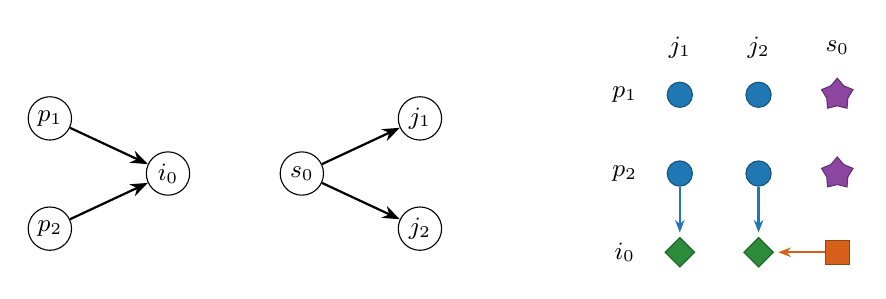
\begin{tikzpicture}[scale=1.0]
 \begin{scope}[yshift=-0.9cm]
  \node[vtx] (p1) at (0,0.7) {$p_1$}; \node[vtx] (p2) at (0,-0.7) {$p_2$};
  \node[vtx] (i0) at (1.5,0) {$i_0$};
  \node[vtx] (s0) at (3.2,0) {$s_0$};
  \node[vtx] (j1) at (4.7,0.7) {$j_1$}; \node[vtx] (j2) at (4.7,-0.7) {$j_2$};
  \draw[arc] (p1)--(i0); \draw[arc] (p2)--(i0); \draw[arc] (s0)--(j1); \draw[arc] (s0)--(j2);
 \end{scope}
 \begin{scope}[xshift=8.0cm,yshift=0.1cm]
  \foreach \x/\l in {0/j_1,1/j_2,2/s_0} \node[font=\small] at (\x,0.6) {$\l$};
  \foreach \y/\l in {0/p_1,-1/p_2,-2/i_0} \node[font=\small] at (-0.7,\y) {$\l$};
  \foreach \x in {0,1,2} \foreach \y in {0,-1,-2} \node[gridpt] at (\x,\y) {};
  \node[Lpt] (r11) at (0,0) {}; \node[Lpt] (r12) at (1,0) {}; \node[Lpt] (r21) at (0,-1) {}; \node[Lpt] (r22) at (1,-1) {};
  \node[Rpt] (c) at (2,-2) {};
  \node[Zpt] at (0,-2) {}; \node[Zpt] at (1,-2) {};
  \node[Hpt] at (2,0) {}; \node[Hpt] at (2,-1) {};
  \draw[famL,-{Stealth[length=1.6mm]},thick] (r21)--(0,-1.75);
  \draw[famL,-{Stealth[length=1.6mm]},thick] (r22)--(1,-1.75);
  \draw[famR,-{Stealth[length=1.6mm]},thick] (c)--(1.25,-2);
 \end{scope}
\end{tikzpicture}
\caption{\Cref{ex:star} with $n=2$; only the rows $p_1,p_2,i_0$ and the
columns $j_1,j_2,s_0$ of the grid are drawn. The four left members (blue)
all conflict with the single right member $c$ (orange). The conflict points
(green) lie in row $i_0$ and the opposite corners (purple) in column $s_0$.
Deleting $c$ removes every conflict at cost $1$; deleting the left members
instead would cost $n^2=4$ against $\abs H=2$.}
\label{fig:star}
\end{figure}

\subsection{Reduction to a matching bound}\label{sec:gamma}

\begin{definition}[The augmented graph]\label{def:gamma}
Let $Z_L$ and $Z_R$ be two disjoint copies of $Z$; write $z_L,z_R$ for the
copies of $z\in Z$. The bipartite graph $\Gamma$ has sides
\[
 \Lp=\Rf\sqcup Z_L,\qquad \Rp=\Cf\sqcup Z_R,
\]
and three kinds of edges:
\begin{itemize}
\item[(E1)] $r\,c$ for every conflicting $r\in\Rf$, $c\in\Cf$ (\emph{conflict edges});
\item[(E2)] $r\,z_R$ whenever $z\in Z$ and $r\in\Rf$ covers $z$;
\item[(E3)] $z_L\,c$ whenever $z\in Z$ and $c\in\Cf$ covers $z$.
\end{itemize}
\end{definition}

Every conflict $(r,c)$ with conflict point $z$ produces the path
$z_L - c - r - z_R$ in $\Gamma$, since both $r$ and $c$ cover $z$
(\cref{fig:gamma}). Different conflicts may share vertices and edges. We
write $\nu(\Gamma)$ for the maximum size of a matching.

\begin{figure}[ht]
\centering
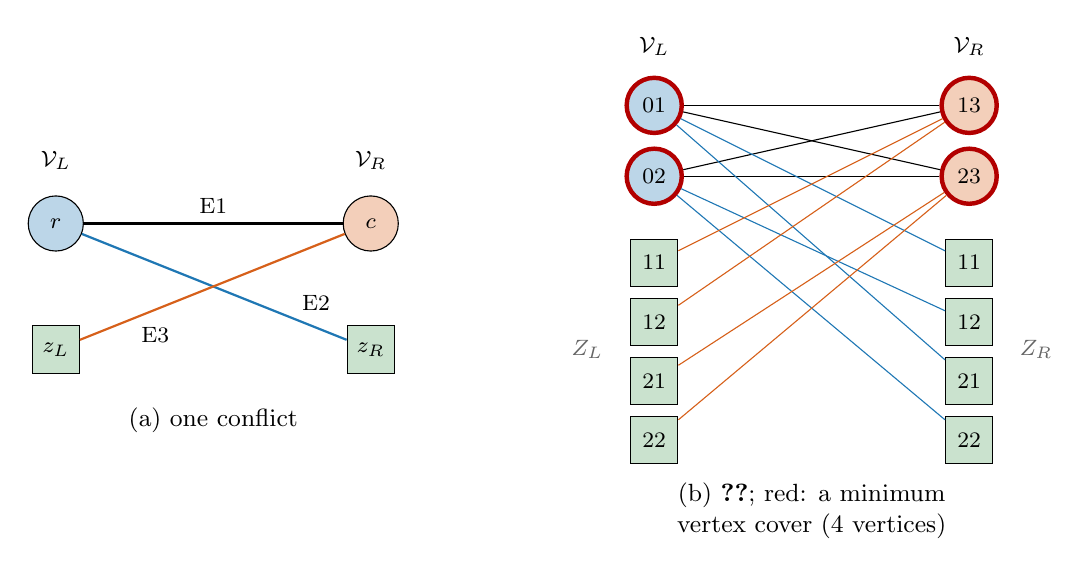
\begin{tikzpicture}[
  ov/.style={circle,draw,inner sep=1pt,minimum size=7mm,font=\footnotesize},
  cv/.style={rectangle,draw,inner sep=1pt,minimum size=6mm,font=\footnotesize}]
 \begin{scope}
  \node[font=\footnotesize] at (1,1.2) {$\Lp$}; \node[font=\footnotesize] at (5,1.2) {$\Rp$};
  \node[ov,fill=famL!30] (r) at (1,0.4) {$r$};
  \node[cv,fill=zcol!25] (zl) at (1,-1.2) {$z_L$};
  \node[ov,fill=famR!30] (c) at (5,0.4) {$c$};
  \node[cv,fill=zcol!25] (zr) at (5,-1.2) {$z_R$};
  \draw[thick] (r) -- node[above,font=\footnotesize] {E1} (c);
  \draw[thick,famL] (r) -- node[pos=0.8,above right=-1pt,font=\footnotesize,black] {E2} (zr);
  \draw[thick,famR] (zl) -- node[pos=0.2,below right=-1pt,font=\footnotesize,black] {E3} (c);
  \node[font=\small] at (3,-2.1) {(a) one conflict};
 \end{scope}
 \begin{scope}[xshift=8.6cm,yshift=1.9cm]
  \node[font=\footnotesize] at (0,0.75) {$\Lp$}; \node[font=\footnotesize] at (4,0.75) {$\Rp$};
  \node[ov,fill=famL!30,ultra thick,draw=red!70!black] (r1) at (0,0) {$01$};
  \node[ov,fill=famL!30,ultra thick,draw=red!70!black] (r2) at (0,-0.9) {$02$};
  \node[ov,fill=famR!30,ultra thick,draw=red!70!black] (c1) at (4,0) {$13$};
  \node[ov,fill=famR!30,ultra thick,draw=red!70!black] (c2) at (4,-0.9) {$23$};
  \foreach \z/\y in {11/-2.0,12/-2.75,21/-3.5,22/-4.25} {
   \node[cv,fill=zcol!25] (L\z) at (0,\y) {$\z$};
   \node[cv,fill=zcol!25] (R\z) at (4,\y) {$\z$};
  }
  \foreach \a in {r1,r2} \foreach \b in {c1,c2} \draw (\a)--(\b);
  \draw[famL] (r1)--(R11); \draw[famL] (r1)--(R21);
  \draw[famL] (r2)--(R12); \draw[famL] (r2)--(R22);
  \draw[famR] (L11)--(c1); \draw[famR] (L12)--(c1);
  \draw[famR] (L21)--(c2); \draw[famR] (L22)--(c2);
  \node[font=\footnotesize,text=black!60] at (-0.85,-3.1) {$Z_L$};
  \node[font=\footnotesize,text=black!60] at (4.85,-3.1) {$Z_R$};
  \node[font=\small,align=center] at (2,-5.15) {(b) \cref{ex:K22}; red: a minimum\\ vertex cover ($4$ vertices)};
 \end{scope}
\end{tikzpicture}
\caption{The augmented graph $\Gamma$. (a) A single conflict $(r,c)$ with
conflict point $z$ forces a path of three edges. (b) The graph for
\cref{ex:K22} (pairs written $ij$). Here $\nu(\Gamma)=4\le\abs Z+\abs H=5$. The
minimum vertex cover consists of the four original members, so the proof
deletes all of them.}
\label{fig:gamma}
\end{figure}

\begin{claim}\label{cl:isolated}
A member of $\Rf\cup\Cf$ that is in no conflict is an isolated vertex of $\Gamma$.
\end{claim}

\begin{proof}
Let $r=(p,j)\in\Rf$ be in no conflict. It has no E1 edges. Suppose it had an E2
edge to $z_R$, with $z=(i,j)\in Z$ and $p\to i$. Since $z\in Z$, some conflict has
conflict point $z$, so there is $(i,s)\in\Cf$ with $s\to j$. But then $r$ and
$(i,s)$ conflict, a contradiction. The argument for $\Cf$ is symmetric.
\end{proof}

\begin{claim}[Covers give prunings]\label{cl:cover-to-pruning}
Let $K$ be a vertex cover of $\Gamma$ (every edge has an endpoint in $K$) that
contains no isolated vertex and has $\abs K\le\abs Z+\abs H$. Then
$\Rf'=\Rf\setminus K$ and $\Cf'=\Cf\setminus K$ satisfy \ref{P1}--\ref{P3}.
\end{claim}

\begin{proof}
\ref{P1}: every conflict edge has an endpoint in $K$, which is deleted.
\ref{P2}: by \cref{cl:isolated} such members are isolated, hence not in $K$.
\ref{P3}: let $Z_{\mathrm{cov}}=Z\cap(\Ff\Rf'\cup\Fs\Cf')$. If $z\in Z_{\mathrm{cov}}$ is
covered by a kept $r\in\Rf'$, then the edge $r\,z_R$ forces $z_R\in K$. If it
is covered by a kept $c\in\Cf'$, then $z_L\in K$. Either way, $K$ contains at
least one copy of each $z\in Z_{\mathrm{cov}}$. So
\[
 \abs{\Rf\setminus\Rf'}+\abs{\Cf\setminus\Cf'}=\abs{K\cap(\Rf\sqcup\Cf)}
 \le\abs K-\abs{Z_{\mathrm{cov}}}\le\abs H+\abs Z-\abs{Z_{\mathrm{cov}}},
\]
and $\abs Z-\abs{Z_{\mathrm{cov}}}$ is the last term of~\eqref{eq:pruning-bound}.
\end{proof}

\begin{claim}[K\H{o}nig]\label{cl:konig}
Every bipartite graph has a vertex cover $K$ with $\abs K=\nu$ that contains
no vertex left unmatched by some fixed maximum matching. In particular $K$
contains no isolated vertex.
\end{claim}

\begin{proof}
This is K\H{o}nig's theorem~\cite{konig1931}. We recall the construction to
check the extra property. Fix a maximum matching $\Mm$. Starting from all
unmatched left vertices, explore \emph{alternating paths}: go from left to
right along non-matching edges and from right to left along matching
edges. Let $W_L,W_R$ be the reached vertices, and put
$K=(\Lp\setminus W_L)\cup W_R$.
No unmatched right vertex is reached, since otherwise we would have an
augmenting path. A matched right vertex that is reached leads to its mate.
A matched left vertex can only be reached through its mate. So the two
ends of a matching edge are both reached or both unreached, and $K$ contains
exactly one end of each matching edge. Hence $\abs K=\abs\Mm$. Unmatched left
vertices are reached and so are not in $K$, and unmatched right vertices are
not reached. Finally, $K$ is a cover. An edge from a reached left vertex to
an unreached right vertex cannot be a non-matching edge (it would have been
followed) or a matching edge (whose ends have the same status).
\end{proof}

By \cref{cl:cover-to-pruning,cl:konig}, the pruning lemma follows from:

\begin{proposition}[Matching bound]\label{prop:matching-bound}
$\nu(\Gamma)\le\abs Z+\abs H$.
\end{proposition}

The rest of this section proves \cref{prop:matching-bound}. If there are no
conflicts, $\Gamma$ has no edges and there is nothing to prove, so we
assume there is at least one conflict.

\subsection{Strategy: three kinds of matching edges}\label{sec:strategy}

Let $\Gamma_L$ be the subgraph of E2 edges (between $\Rf$ and $Z_R$) and
$\Gamma_N$ the subgraph of E3 edges (between $Z_L$ and $\Cf$). Fix a maximum
matching $\Mm$ of $\Gamma$ that has, among all maximum matchings, the fewest
conflict edges. Split it as
\[
 \Mm=\underbrace{\Mm_1}_{k\text{ conflict edges}}\ \sqcup\ \underbrace{\alpha}_{\ell\text{ edges of }\Gamma_L}\ \sqcup\ \underbrace{\beta}_{t\text{ edges of }\Gamma_N},
 \qquad \nu(\Gamma)=k+\ell+t,
\]
and let $R_\alpha\subseteq\Rf$, $C_\beta\subseteq\Cf$ be the original members matched
by $\alpha$, respectively $\beta$ (\cref{fig:decomposition}). Let $R_1\subseteq\Rf$ and $C_1\subseteq\Cf$ be
the left and right ends of the conflict edges in $\Mm_1$. Then
$\abs{R_1}=\abs{C_1}=k$, and $R_1\cap R_\alpha=\varnothing$, $C_1\cap C_\beta=\varnothing$,
since a vertex is matched only once.

\begin{figure}[ht]
\centering
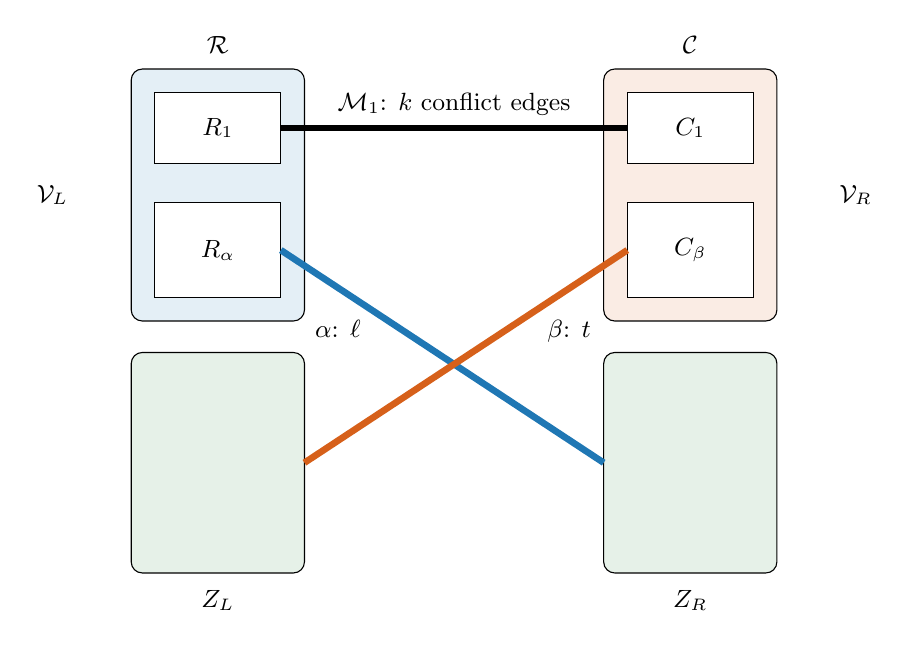
\begin{tikzpicture}[font=\small]
 \draw[rounded corners,fill=famL!12] (0,0) rectangle (2.2,3.2); \node at (1.1,3.5) {$\Rf$};
 \draw[rounded corners,fill=zcol!12] (0,-3.2) rectangle (2.2,-0.4); \node at (1.1,-3.55) {$Z_L$};
 \draw[rounded corners,fill=famR!12] (6,0) rectangle (8.2,3.2); \node at (7.1,3.5) {$\Cf$};
 \draw[rounded corners,fill=zcol!12] (6,-3.2) rectangle (8.2,-0.4); \node at (7.1,-3.55) {$Z_R$};
 \node at (-1.0,1.6) {$\Lp$}; \node at (9.2,1.6) {$\Rp$};
 % R1 and R_alpha
 \draw[fill=white] (0.3,2.0) rectangle (1.9,2.9); \node at (1.1,2.45) {$R_1$};
 \draw[fill=white] (0.3,0.3) rectangle (1.9,1.5); \node at (1.1,0.9) {$R_\alpha$};
 \draw[fill=white] (6.3,2.0) rectangle (7.9,2.9); \node at (7.1,2.45) {$C_1$};
 \draw[fill=white] (6.3,0.3) rectangle (7.9,1.5); \node at (7.1,0.9) {$C_\beta$};
 \draw[line width=2.4pt] (1.9,2.45) -- node[above] {$\Mm_1$: $k$ conflict edges} (6.3,2.45);
 \draw[line width=2.4pt,famL] (1.9,0.9) -- node[pos=0.28,below left=-1pt,black] {$\alpha$: $\ell$} (6.0,-1.8);
 \draw[line width=2.4pt,famR] (2.2,-1.8) -- node[pos=0.72,below right=-1pt,black] {$\beta$: $t$} (6.3,0.9);
\end{tikzpicture}
\caption{The three kinds of edges in the maximum matching $\Mm$: conflict
edges (black), edges of $\Gamma_L$ from $\Rf$ to $Z_R$ (blue) and edges of
$\Gamma_N$ from $Z_L$ to $\Cf$ (orange). The linear algebra handles $\ell$ and $t$
by the ranks of two matrices $L,N$, and $k$ by vectors of $\ker L$ that
survive under $B$.}
\label{fig:decomposition}
\end{figure}

\begin{claim}\label{cl:alpha-max}
$\alpha$ is a maximum matching of $\Gamma_L$, and $\beta$ is a maximum matching of $\Gamma_N$.
\end{claim}

\begin{proof}
If $\alpha$ were not maximum in $\Gamma_L$, there would be an $\alpha$-augmenting
path $\pi$ in $\Gamma_L$, from an $\alpha$-unmatched $r\in\Rf$ to an $\alpha$-unmatched
$z_R\in Z_R$. The vertex $z_R$ is unmatched in $\Mm$ too, because all its
neighbors are in $\Rf$, so any $\Mm$-edge at $z_R$ would belong to $\alpha$.
The interior vertices of $\pi$ are matched by $\alpha\subseteq\Mm$. If $r$ is
unmatched in $\Mm$, then $\pi$ is $\Mm$-augmenting, contradicting maximality.
Otherwise $r$ is matched in $\Mm$ by a conflict edge. Removing that edge and
augmenting along $\pi$ gives a maximum matching with fewer conflict edges,
contradicting the choice of $\Mm$. The argument for $\beta$ is symmetric.
\end{proof}

\paragraph{The plan.}
We will put real numbers on the arrows of the relation and build four
matrices $L,N,A,B$ (\cref{sec:matrices}). We will show:
\begin{itemize}
\item the identity $NL=AB$ makes
$\RR^{\Rf}\to\RR^Z\oplus\RR^H\to\RR^{\Cf}$ a \emph{complex}, so the ranks of
its two maps add up to at most $\abs Z+\abs H$ (\cref{sec:rank});
\item $\rank L=\ell$ and $\rank N=t$, using Edmonds' principle that a generic
matrix with prescribed zero pattern has rank equal to the maximum matching
size (\cref{sec:generic});
\item the $k$ conflict edges of $\Mm_1$ add $k$ dimensions to the first
map, through vectors of $\ker L$ that $B$ keeps independent; this uses a
kernel lemma (\cref{sec:kernel}).
\end{itemize}
Together: $\nu(\Gamma)=k+\ell+t\le\abs Z+\abs H$.

\subsection{Four matrices and two factorizations}\label{sec:matrices}

For every arrow $x\to y$ of the relation, introduce two variables $a_{xy}$ and
$b_{xy}$, all distinct. When $x\not\to y$ we set $a_{xy}=b_{xy}=0$. For an
assignment of real values we define four matrices, with rows and columns
indexed by the sets shown:
\[
\begin{array}{ll}
 L\in\RR^{Z\times\Rf}, & L_{(i,j),(p,j)}=a_{pi},\\[2pt]
 N\in\RR^{\Cf\times Z}, & N_{(i,s),(i,j)}=b_{sj},
\end{array}\qquad
\begin{array}{ll}
 B\in\RR^{H\times\Rf}, & B_{(p,s),(p,j)}=b_{sj},\\[2pt]
 A\in\RR^{\Cf\times H}, & A_{(i,s),(p,s)}=a_{pi},
\end{array}
\]
and all entries not of the indicated form (for example
$L_{(i,j),(p,j')}$ with $j\ne j'$) are $0$. In words, the $a$-matrices $L$ and
$A$ move the first coordinate forward along $p\to i$, and the $b$-matrices
$N$ and $B$ move the second coordinate backward along $s\to j$.

\begin{figure}[ht]
\centering
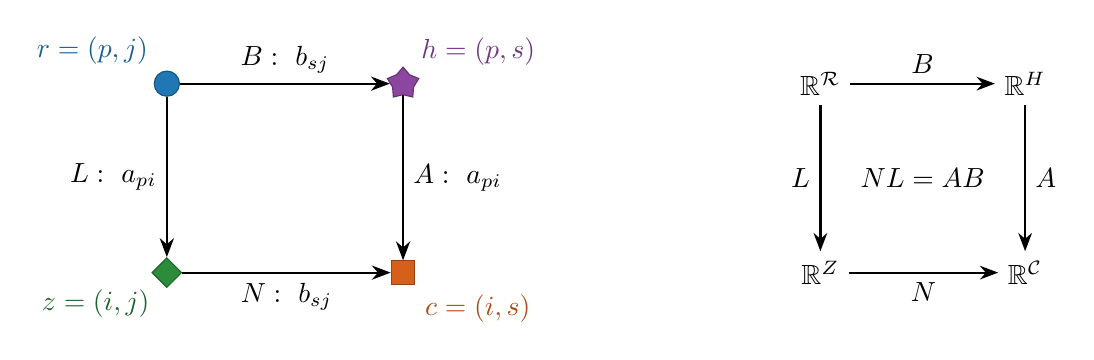
\begin{tikzpicture}
 \begin{scope}
  \node[Lpt,label={[famL!80!black]above left:$r=(p,j)$}] (r) at (0,0) {};
  \node[Hpt,label={[hcol!80!black]above right:$h=(p,s)$}] (h) at (3,0) {};
  \node[Zpt,label={[zcol!70!black]below left:$z=(i,j)$}] (z) at (0,-2.4) {};
  \node[Rpt,label={[famR!80!black]below right:$c=(i,s)$}] (c) at (3,-2.4) {};
  \draw[-{Stealth[length=2.4mm]},thick] (r) -- node[left] {$L:\ a_{pi}$} (z);
  \draw[-{Stealth[length=2.4mm]},thick] (z) -- node[below] {$N:\ b_{sj}$} (c);
  \draw[-{Stealth[length=2.4mm]},thick] (r) -- node[above] {$B:\ b_{sj}$} (h);
  \draw[-{Stealth[length=2.4mm]},thick] (h) -- node[right] {$A:\ a_{pi}$} (c);
 \end{scope}
 \begin{scope}[xshift=8.3cm,yshift=-1.2cm]
  \node (RR) at (0,1.2) {$\RR^{\Rf}$};
  \node (RH) at (2.6,1.2) {$\RR^{H}$};
  \node (RZ) at (0,-1.2) {$\RR^{Z}$};
  \node (RC) at (2.6,-1.2) {$\RR^{\Cf}$};
  \draw[-{Stealth},thick] (RR) -- node[left] {$L$} (RZ);
  \draw[-{Stealth},thick] (RZ) -- node[below] {$N$} (RC);
  \draw[-{Stealth},thick] (RR) -- node[above] {$B$} (RH);
  \draw[-{Stealth},thick] (RH) -- node[right] {$A$} (RC);
  \node at (1.3,0) {$NL=AB$};
 \end{scope}
\end{tikzpicture}
\caption{The two routes from a left member $r$ to a right member $c$. Via the
conflict point $z$ (first change the first coordinate, then the second), or
via the opposite corner $h$ (the other order). For a conflicting pair both
routes give the entry $a_{pi}b_{sj}$, and for a non-conflicting pair both
give $0$. This is the identity $NL=AB$. The corners sit at their true
grid positions (rows $p,i$; columns $j,s$), and the diagram on the right
has the same shape. Arrows show the direction of the
linear maps. $L$ and $A$ follow the arc $p\to i$, while $N$ and $B$ run
\emph{against} the arc $s\to j$, unlike the set operator $\Fs$ in
\cref{fig:coord}.}
\label{fig:square}
\end{figure}

\begin{claim}\label{cl:supports}
The variable entries of $L$ (those not identically zero) sit exactly on the
edges of $\Gamma_L$, and those of $N$ exactly on the edges of $\Gamma_N$.
\end{claim}

\begin{proof}
$L_{z,r}$ with $z=(i,j)$, $r=(p,j)$ is the variable $a_{pi}$ if $p\to i$, i.e.\
if $r$ covers $z$, and is $0$ otherwise. Similarly $N_{c,z}$ with $c=(i,s)$,
$z=(i,j)$ is $b_{sj}$ exactly when $s\to j$, i.e.\ when $c$ covers $z$.
\end{proof}

\begin{claim}[Two factorizations]\label{cl:commute}
For every assignment, $NL=AB$. Both products have entry $a_{pi}b_{sj}$ at
position $(c,r)$ if $r=(p,j)$ and $c=(i,s)$ conflict, and $0$ otherwise.
\end{claim}

\begin{proof}
$(NL)_{c,r}=\sum_{z\in Z}N_{c,z}L_{z,r}$. A nonzero term needs $z$ in row $i$
(for $N$) and in column $j$ (for $L$), so $z=(i,j)$, and then the term is
$b_{sj}a_{pi}$. If $r,c$ conflict, then $(i,j)\in Z$ and the entry is
$a_{pi}b_{sj}$. If not, then $p\not\to i$ or $s\not\to j$, and the product is $0$.
Likewise $(AB)_{c,r}=\sum_{h\in H}A_{c,h}B_{h,r}$ has at most one term,
$h=(p,s)$, with value $a_{pi}b_{sj}$. If $r,c$ conflict, then $(p,s)\in H$. If
not, the value is $0$.
\end{proof}

The matrix $NL=AB$ might be called the \emph{conflict matrix}: it is
supported on the conflict edges. The first factorization passes through
$\RR^Z$ and the second through $\RR^H$. The whole proof plays these two
against each other.

\begin{remark}[The four matrices are two commuting operators]\label{rem:kronecker}
There is a structural reason for \cref{cl:commute}. Let
$\mathsf a,\mathsf b\in\RR^{X\times X}$ be the matrices of the variables,
$(\mathsf a)_{xy}=a_{xy}$ and $(\mathsf b)_{xy}=b_{xy}$ (zero off the relation),
and consider the two operators on $\RR^{X\times X}$, with coordinates
indexed by grid points,
\[
 (\mathcal A x)_{(i,j)}=\sum_{p}a_{pi}\,x_{(p,j)},\qquad
 (\mathcal B x)_{(i,s)}=\sum_{j}b_{sj}\,x_{(i,j)} .
\]
In Kronecker notation $\mathcal A=\mathsf a^{\T}\otimes I$ and
$\mathcal B=I\otimes\mathsf b$: $\mathcal A$ moves the first coordinate
forward along the relation and $\mathcal B$ moves the second coordinate
backward. They are the linear versions of $\Ff$ and of $\Fs$ for the
reversed relation, and they \emph{commute},
$\mathcal A\mathcal B=\mathcal B\mathcal A=\mathsf a^{\T}\otimes\mathsf b$,
simply because they act on different coordinates. This is the linear
shadow of $\Ff\Fs=\Fs\Ff$. The four matrices are restrictions of these
two: $L$ and $A$ are $\mathcal A$ with rows and columns restricted to
$Z\times\Rf$ and $\Cf\times H$, while $N$ and $B$ are $\mathcal B$
restricted to $\Cf\times Z$ and $H\times\Rf$. The $(c,r)$ entry of
$\mathcal B\mathcal A$ is a single term, with middle index $z=(i,j)$, and
the $(c,r)$ entry of $\mathcal A\mathcal B$ is a single term with middle
index $h=(p,s)$; both equal $a_{pi}b_{sj}$. When this is nonzero $r$ and
$c$ conflict, so $z\in Z$ and $h\in H$, and restricting the middle index to
$Z$, respectively $H$, loses nothing. That is $NL=AB$. The whole of
\cref{sec:pruning} can thus be read as linear algebra on the grid, with the
same two commuting moves as in \cref{sec:pairs}.
\end{remark}

\subsection{A three-term complex}\label{sec:rank}

The identity $NL=AB$ says that the square in \cref{fig:square} commutes.
Put the two routes side by side: the maps
\[
 \LB:\RR^{\Rf}\to\RR^{Z}\oplus\RR^{H},\qquad
 \NmA:\RR^{Z}\oplus\RR^{H}\to\RR^{\Cf}
\]
compose to $NL-AB=0$. In other words,
\begin{equation}\label{eq:complex}
 \RR^{\Rf}\xrightarrow{\ \LB\ }\RR^{Z}\oplus\RR^{H}\xrightarrow{\ \NmA\ }\RR^{\Cf}
\end{equation}
is a \emph{complex}: the image of the first map lies in the kernel of the
second.

\begin{claim}[Dimension count]\label{cl:rank-inequality}
For every assignment, $\rank\LB+\rank\NA\le\abs Z+\abs H$.
\end{claim}

\begin{proof}
By~\eqref{eq:complex} and rank--nullity for the second map,
$\rank\LB\le\dim\ker\NmA=\abs Z+\abs H-\rank\NmA$, and
$\rank\NmA=\rank\NA$, since changing the sign of a block of columns does
not change the rank.
\end{proof}

So \cref{prop:matching-bound} follows once we find an assignment with
\begin{equation}\label{eq:two-lower-bounds}
 \rank\LB\ \ge\ \ell+k\qquad\text{and}\qquad \rank\NA\ \ge\ t .
\end{equation}
The second inequality only needs $\rank N=t$, as $N$ is a submatrix of
$\NA$. In the first, $\ell$ comes from $\rank L=\ell$, and the remaining
$k$ dimensions come from the conflict edges of $\Mm_1$: each gives a vector
of $\ker L$ that $B$ does not kill, and these images stay independent. The
next two subsections provide the assignment and the vectors.

\begin{remark}
The original preprint counts in two steps, with rank--nullity for $A$ and
Sylvester's inequality $\rank(NL)\ge\rank L+\rank N-\abs Z$, placing the
$k$ extra dimensions in $\ker A$, where $B$ sends $\ker L$ because
$AB=NL$. The complex~\eqref{eq:complex} packages both steps into
\cref{cl:rank-inequality}, and $\ker A$ is no longer needed. The Lean
formalization follows the two-step count.
\end{remark}

\subsection{Choosing the coefficients}\label{sec:generic}

We use three elementary facts about real polynomials in finitely many
variables. (i)~A product of nonzero polynomials is nonzero. (ii)~A nonzero
polynomial is nonzero at some real point (induction on the number of
variables: a nonzero univariate polynomial has finitely many roots).
(iii)~Let $\Phi$ be a square matrix whose entries are $0$ or variables, with
\emph{distinct} variables in distinct positions. If the positions of the
variables contain a perfect matching (a permutation $\sigma$ with all
$\Phi_{x,\sigma(x)}$ variables), then $\det\Phi\ne0$. Indeed, distinct
permutations give products of distinct sets of variables, so the monomial of
$\sigma$ cannot cancel.

\begin{claim}[Generic rank of $L$ and $N$]\label{cl:edmonds}
\begin{enumerate}[label=(\alph*)]
\item For every assignment, $\rank L\le\ell$ and $\rank N\le t$.
\item The square submatrix of $L$ with columns $R_\alpha$ and rows
$\{z:z_R\text{ is matched by }\alpha\}$ has a determinant that is a nonzero
polynomial. The same holds for the submatrix of $N$ with rows $C_\beta$ and
columns $\{z: z_L\text{ is matched by }\beta\}$.
\end{enumerate}
\end{claim}

\begin{proof}
(a) If a square submatrix of $L$ has nonzero determinant, some term of its
Leibniz expansion is nonzero. That term is a bijection between its rows and
columns using only nonzero entries, that is, by \cref{cl:supports}, a
matching in $\Gamma_L$. So $\rank L\le\nu(\Gamma_L)=\ell$ by \cref{cl:alpha-max}.
Likewise for $N$.

(b) Entries of $L$ vanish unless row and column have the same second
coordinate $j$. So after grouping rows and columns by $j$, the submatrix is
block diagonal, and each block is square because $\alpha$ matches $(p,j)$ with
some $(i,j)$. Within the block of a fixed $j$, the entry in row $(i,j)$ and
column $(p,j)$ is $a_{pi}$, so distinct positions carry distinct variables
(the same variable may reappear in \emph{other} blocks, but this is
harmless). The edges of $\alpha$ give a perfect matching of every block. By
(iii) every block determinant is a nonzero polynomial, and by (i) so is
their product. For $N$ group by the first coordinate $i$ instead, where the
entries $b_{sj}$ in a block are again distinct.
\end{proof}

We need one more family of rank conditions, which are used in
\cref{sec:kernel}. For every arrow $p\to i$ let
\[
 J_p=\{j:(p,j)\in\Rf\},\qquad S_i=\{s:(i,s)\in\Cf\},\qquad
 \Phi^{p,i}=\bigl(b_{sj}\bigr)_{s\in S_i,\ j\in J_p},
\]
a matrix whose entry is the variable $b_{sj}$ when $s\to j$ and $0$
otherwise. (In the original preprint this matrix is called $D^{p,i}$.) Its
variables are distinct. Let $\rho^{p,i}$ be the largest rank it attains over
all real assignments. At an assignment attaining it, some
$\rho^{p,i}\times\rho^{p,i}$ minor is nonzero, so that minor is a nonzero
polynomial (the empty minor, equal to $1$, if $\rho^{p,i}=0$).

\begin{claim}[A simultaneous choice]\label{cl:simultaneous}
There is a real assignment of all variables at which
\begin{enumerate}[label=(\alph*)]
\item the columns of $L$ indexed by $R_\alpha$ form a basis of $\im L$, and $\rank L=\ell$;
\item the rows of $N$ indexed by $C_\beta$ form a basis of the row space of $N$, and $\rank N=t$;
\item every $\Phi^{p,i}$ has its maximum possible rank $\rho^{p,i}$.
\end{enumerate}
\end{claim}

\begin{proof}
Multiply the two polynomials of \cref{cl:edmonds}(b) and one maximal nonzero
minor of each $\Phi^{p,i}$. This is a finite product of nonzero polynomials,
hence nonzero by (i), and by (ii) it is nonzero at some real point. There, the
$\ell$ columns $R_\alpha$ of $L$ are linearly independent, and since
$\rank L\le\ell$ they span $\im L$. Similarly for $N$. Each $\Phi^{p,i}$ has a
nonzero minor of size $\rho^{p,i}$, so its rank is (at least, hence exactly)
$\rho^{p,i}$.
\end{proof}

\emph{From now on we fix such an assignment.} Different conditions share
variables (for example, $b_{sj}$ appears in $N$, in $B$ and in several
$\Phi^{p,i}$). The point of multiplying the polynomials is that all
conditions hold \emph{at the same time}.

\subsection{The kernel lemma and the bound on \texorpdfstring{$\ker A$}{ker A}}\label{sec:kernel}

\begin{lemma}[Kernel lemma; Lemma~3.2 of the original]\label{lem:kernel}
Let $\Phi\in\RR^{S\times J}$ have the maximum rank among all real matrices
whose nonzero entries lie in a given set $T\subseteq S\times J$, and suppose
$\Phi$ itself is supported in $T$. If $x\in\ker\Phi$ and $y\in\ker\Phi^\T$, then
$x_jy_s=0$ for every $(s,j)\in T$.
\end{lemma}

\begin{proof}
Suppose $x_jy_s\ne0$ for some $(s,j)\in T$, and let $\Phi'=\Phi+\gamma e_se_j^\T$ with
$\gamma\ne0$. It is still supported in $T$. Now $\Phi'x=\gamma x_je_s$, so
$e_s\in\im\Phi'$. Also, for every $w$, $\Phi w=\Phi'w-\gamma w_je_s\in\im\Phi'$, so
$\im\Phi\subseteq\im\Phi'$. But $e_s\notin\im\Phi$, because $y$ is orthogonal to
$\im\Phi$ and $y_s\ne0$. Hence $\rank\Phi'>\rank\Phi$, a contradiction.
\end{proof}

\begin{example}
Let $T=\{(1,1),(2,1)\}$ in a $2\times2$ matrix (column $2$ is forced to be
zero) and $\Phi=\begin{psmallmatrix}1&0\\1&0\end{psmallmatrix}$, of the maximum rank $1$. Then
$\ker\Phi=\langle e_2\rangle$ and $\ker\Phi^\T=\langle(1,-1)\rangle$. The pairs
$(s,j)\in T$ have $j=1$, and $x_1=0$ for all $x\in\ker\Phi$, as the lemma predicts.
For the non-generic $\Phi=\begin{psmallmatrix}1&1\\1&1\end{psmallmatrix}$ on the full support (maximum
rank $2$) the conclusion fails: $x=y=(1,-1)$.
\end{example}

So at a generic point the left and right kernels ``avoid each other'' on
the support. We apply this to the matrices $\Phi^{p,i}$.

\begin{remark}[What the kernel lemma says combinatorially]\label{rem:DM}
Read $T$ as a bipartite graph between the rows $S$ and the columns $J$, and
call a column \emph{inessential} if some maximum matching of $T$ misses it;
likewise for rows. If $x\in\ker\Phi$ and $x_j\ne0$, then column $j$ of
$\Phi$ is a combination of the other columns, so deleting it does not lower
the rank. The matrix without column $j$ is supported in $T\setminus\{j\}$,
so its rank is at most $\nu(T\setminus\{j\})$ by the Leibniz argument of
\cref{cl:edmonds}(a), while $\rank\Phi=\nu(T)$. Hence
$\nu(T\setminus\{j\})=\nu(T)$: some maximum matching misses $j$. So
$\ker\Phi$ is supported on inessential columns and $\ker\Phi^\T$ on
inessential rows, and \cref{lem:kernel} says: \emph{there is no edge of
$T$ between an inessential row and an inessential column.} This is a
basic fact of matching theory, part of the Dulmage--Mendelsohn
decomposition of a bipartite graph~\cite{DulmageMendelsohn1958,LovaszPlummer1986},
and the perturbation argument above is a quick proof of it. Only the
maximum rank is needed, not that the entries be generic. In
\cref{cl:conflict-kernel} the graph is the relation $s\to j$ between
$S_i$ and $J_p$, and a conflict $(r,c)$ is one of its edges.
\end{remark}

\begin{claim}[Kernels separate conflicts]\label{cl:conflict-kernel}
For every $u\in\ker B$, every $v\in\ker N^\T$, and every conflicting pair
$r\in\Rf$, $c\in\Cf$,
\[
 u_r\,v_c=0 .
\]
\end{claim}

\begin{proof}
Let $r=(p,j)$ and $c=(i,s)$, so $p\to i$ and $s\to j$. Consider
$\Phi=\Phi^{p,i}$ and the restrictions
\[
 x=(u_{(p,j')})_{j'\in J_p}\in\RR^{J_p},\qquad y=(v_{(i,s')})_{s'\in S_i}\in\RR^{S_i}.
\]
\emph{$x\in\ker\Phi$.} Take a row $s'\in S_i$. If no $j'\in J_p$ has $s'\to j'$, the
row of $\Phi$ is zero. Otherwise, pick such $j'$. Then $(p,j')\in\Rf$ and
$(i,s')\in\Cf$ conflict, so $(p,s')\in H$, and the $(p,s')$ coordinate of
$Bu=0$ reads
\[
 0=(Bu)_{(p,s')}=\sum_{j'\in J_p}b_{s'j'}\,u_{(p,j')}=(\Phi x)_{s'}.
\]
\emph{$y\in\ker\Phi^\T$.} Take a column $j'\in J_p$. If no $s'\in S_i$ has $s'\to j'$,
the column is zero. Otherwise such a conflict gives $(i,j')\in Z$, and the
$(i,j')$ coordinate of $N^\T v=0$ reads
\[
 0=(N^\T v)_{(i,j')}=\sum_{s'\in S_i}b_{s'j'}\,v_{(i,s')}=(\Phi^\T y)_{j'}.
\]
By \cref{cl:simultaneous}(c), $\Phi$ has maximum rank on its support, and
$(s,j)$ is in the support since $s\to j$. By \cref{lem:kernel},
$x_jy_s=u_rv_c=0$.
\end{proof}

Note that \cref{lem:kernel} is applied at the fixed assignment. The
perturbation in its proof is only a thought experiment about $\Phi^{p,i}$
and does not change any of the other matrices.

\begin{claim}\label{cl:kerA}
$\rank\LB\ge\ell+k$.
\end{claim}

\begin{proof}
Let $(r,c)\in\Mm_1$ be a conflict edge of the matching. Since $r\notin R_\alpha$,
\cref{cl:simultaneous}(a) lets us write $Le_r$ as a combination of the
columns $Le_a$, $a\in R_\alpha$. That is, there is a vector
\[
 u^r=e_r+\sum_{a\in R_\alpha}\lambda^r_ae_a\in\ker L .
\]
Similarly, since $c\notin C_\beta$, \cref{cl:simultaneous}(b) gives
$v^c=e_c+\sum_{b\in C_\beta}\mu^c_be_b\in\ker N^\T$, with $v^c_c=1$.

We claim that the $\ell+k$ vectors
\[
 \LB e_a=(Le_a,Be_a)\quad(a\in R_\alpha),\qquad
 \LB u^r=(0,Bu^r)\quad(r\in R_1)
\]
are linearly independent. Suppose
$\sum_{a\in R_\alpha}\theta_a\LB e_a+\sum_{r\in R_1}\theta_r\LB u^r=0$.
The $\RR^Z$-components give $\sum_a\theta_aLe_a=0$, and the columns $Le_a$,
$a\in R_\alpha$, are independent by \cref{cl:simultaneous}(a), so every
$\theta_a=0$. The $\RR^H$-components then give $\sum_r\theta_rBu^r=0$, that
is, $u=\sum_{r\in R_1}\theta_ru^r\in\ker B$. For each $r\in R_1$, with
partner $c$ in $\Mm_1$, \cref{cl:conflict-kernel} applied to $u$ and $v^c$
gives $u_r=u_rv^c_c=0$. But $u_r=\theta_r$, because $u^{r'}$ is supported on
$\{r'\}\cup R_\alpha$ and $R_1\cap R_\alpha=\varnothing$. So all $\theta_r=0$.
\end{proof}

\begin{proof}[Proof of \cref{prop:matching-bound} and of \cref{lem:pruning}]
At the assignment fixed after \cref{cl:simultaneous} we have $\rank N=t$,
and $\rank\LB\ge\ell+k$ by \cref{cl:kerA}. By \cref{cl:rank-inequality},
\[
 \nu(\Gamma)=k+\ell+t\ \le\ \rank\LB+\rank\NA\ \le\ \abs Z+\abs H .
\]
\Cref{cl:konig} gives a vertex cover of this size with no isolated vertex,
and \cref{cl:cover-to-pruning} turns it into the required pruning.
\end{proof}

\begin{idea}[Summary of the pruning lemma]
The matching bound is the heart of the matter. Because $\Ff$ and $\Fs$
commute, the conflict matrix factors through $\RR^Z$ and through $\RR^H$,
$NL=AB$, and this makes $\RR^{\Rf}\to\RR^Z\oplus\RR^H\to\RR^{\Cf}$ a
complex: the ranks of its two maps add up to at most $\abs Z+\abs H$. A
maximum matching of $\Gamma$ certifies lower bounds for these ranks:
$\ell$ edges through $L$ and $t$ edges through $N$ (generic rank $=$
matching number), and $k$ conflict edges, each contributing a vector of
$\ker L$ whose image under $B$ is new. The kernel lemma keeps these images
independent.
\end{idea}

\begin{remark}[Towards a combinatorial proof?]\label{rem:combinatorial}
Neither orientation nor linear algebra appears in the \emph{statement} of
\cref{prop:matching-bound}, and one may ask for a proof by alternating
paths. Here is what a maximum matching sees. With the notation of
\cref{sec:strategy}, let $Z_\alpha$ and $Z_\beta$ be the sets of $z\in Z$
whose copies $z_R$, respectively $z_L$, are matched by $\Mm$. Then
\[
 \nu(\Gamma)=k+\abs{Z_\alpha}+\abs{Z_\beta}
 =k+\abs{Z_\alpha\cup Z_\beta}+\abs{Z_\alpha\cap Z_\beta},
\]
so the bound would follow from $k+\abs{Z_\alpha\cap Z_\beta}\le\abs H$.
Each of the $k+\abs{Z_\alpha\cap Z_\beta}$ objects on the left comes with
an opposite corner: a conflict edge $(r,c)$ has its $h$, and a doubly
matched $z$ is matched to some $r_z$ and some $c_z$, which both cover $z$
and therefore conflict, with a corner $h_z$. If these corners were always
distinct we would be done. They need not be, and the inequality can fail
for a maximum matching with the fewest conflict edges. In a computer
search over about $5000$ random instances with small $\Gamma$ (the folder
\texttt{experiments/}), there was always \emph{some} maximum matching
satisfying $k+\abs{Z_\alpha\cap Z_\beta}\le\abs H$. Whether this holds in
general, and whether it has a direct proof, we do not know. The kernel
lemma itself has a combinatorial meaning (\cref{rem:DM}); the place where
linear algebra seems essential is the \emph{sum} $\sum_r\theta_ru^r$ in the
proof of \cref{cl:kerA}, which handles several alternating structures at
once.
\end{remark}

\section{The contradiction}\label{sec:contradiction}

\begin{idea}[What this section does]
We carry out the plan of \cref{sec:ledger}. The graph $G$ only needs
properties (G1) and (G2) from the end of \cref{sec:reduction}. All the
checks below are short ``two-step path'' arguments in the grid. The one
non-trivial input is the pruning lemma.
\end{idea}

\begin{proposition}[Proposition~4.1 of the original]\label{prop:no-concave}
There is no nonempty oriented graph $G$ in which every vertex has an
in-neighbor and
\begin{equation}\label{eq:concave-again}
 \abs U+\abs{F^2(U)}<2\abs{F(U)}\qquad\text{for every }\varnothing\ne U\subsetneq V(G).
\end{equation}
\end{proposition}

\begin{proof}
Suppose $G$ is such a graph, let $X=V(G)$, and use the arc relation of $G$ in
the definitions of \cref{sec:pairs}. By \cref{lem:diag-compatible} we can fix
an admissible pair $(P,Q)$ of maximum value. Write
\[
 \mu=\abs P+\abs Q,\qquad d=\unc(P,Q)=\abs X^2-\abs{\Ff P}-\abs{\Fs Q}.
\]
The proof is a sequence of claims.

\begin{claim}\label{cl:lines-proper}
Every column $P_j$ and every row $Q_i$ is a nonempty proper subset of $X$.
\end{claim}

\begin{proof}
$j\in P_j$ and $i\in Q_i$ because $\Delta\subseteq P\cap Q$. Suppose $P_j=X$. Every
vertex has an in-neighbor, so $F(X)=X$ and column $j$ of $\Ff P$ is all of
$X$ by~\eqref{eq:columnwise}. Choose $w\to j$. Then $(w,w)\in Q$ gives
$(w,j)\in\Fs Q$, while $(w,j)\in\Ff P$, contradicting compatibility. If $Q_i=X$, then
row $i$ of $\Fs Q$ is all of $X$. For $w\to i$, $(w,w)\in P$ gives $(i,w)\in\Ff P$, again a
contradiction.
\end{proof}

\begin{claim}\label{cl:fiber-sums}
$\abs P+\abs{\Ff^2P}<2\abs{\Ff P}$ and $\abs Q+\abs{\Fs^2Q}<2\abs{\Fs Q}$.
\end{claim}

\begin{proof}
Apply~\eqref{eq:concave-again} to each column $U=P_j$, which is allowed by
\cref{cl:lines-proper}, and sum over the $\abs X\ge1$ columns
using~\eqref{eq:columnwise}:
\begin{equation}\label{eq:fiber-sum}
 \abs P+\abs{\Ff^2P}=\sum_j\bigl(\abs{P_j}+\abs{F^2(P_j)}\bigr)<\sum_j2\abs{F(P_j)}=2\abs{\Ff P}.
\end{equation}
The same argument over the rows of $Q$ gives the second inequality.
\end{proof}

Now define the new families as complements of the second iterated images:
\[
 \Rf=(X\times X)\setminus\Fs^2Q,\qquad\Cf=(X\times X)\setminus\Ff^2P .
\]
Note the swap: the new \emph{left} family is built from the old \emph{right} one.

\begin{claim}[Gain]\label{cl:gain}
$\abs\Rf+\abs\Cf>\mu+2d$.
\end{claim}

\begin{proof}
By \cref{cl:fiber-sums},
$\abs\Rf+\abs\Cf=2\abs X^2-\abs{\Fs^2Q}-\abs{\Ff^2P}
>2\abs X^2+\abs P+\abs Q-2\abs{\Ff P}-2\abs{\Fs Q}=\mu+2d$.
\end{proof}

\begin{figure}[ht]
\centering
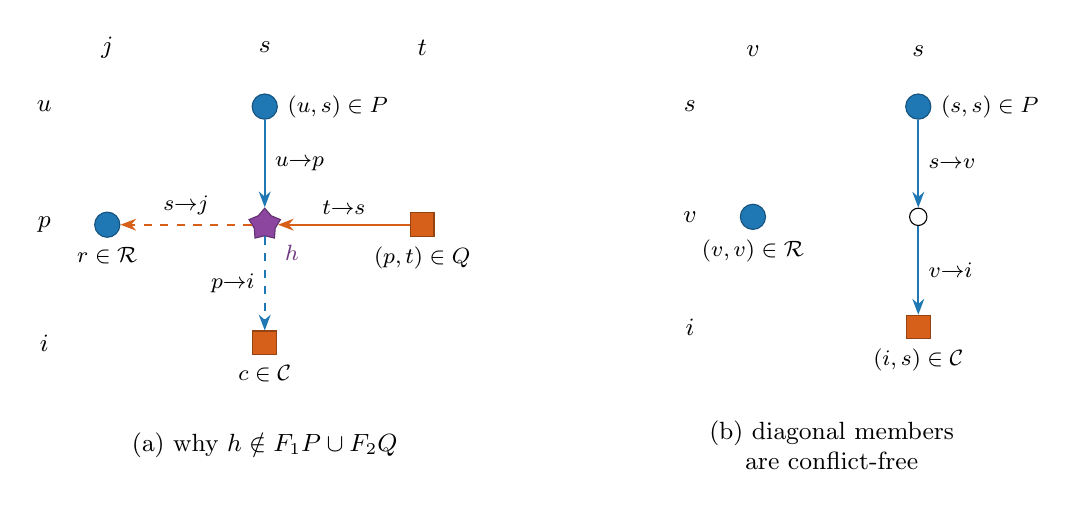
\begin{tikzpicture}[scale=1.0]
 \begin{scope}
  \node[font=\small] at (0,0.75) {$j$}; \node[font=\small] at (2.0,0.75) {$s$}; \node[font=\small] at (4.0,0.75) {$t$};
  \node[font=\small] at (-0.8,0) {$u$}; \node[font=\small] at (-0.8,-1.5) {$p$}; \node[font=\small] at (-0.8,-3.0) {$i$};
  \foreach \x/\y in {2.0/0,0/-1.5,2.0/-1.5,4.0/-1.5,2.0/-3.0} \node[gridpt] at (\x,\y) {};
  \node[Lpt,label={[font=\footnotesize]right:$(u,s)\in P$}] (us) at (2.0,0) {};
  \node[Hpt,label={[font=\footnotesize,hcol!80!black]below right:$h$}] (h) at (2.0,-1.5) {};
  \node[Rpt,label={[font=\footnotesize]below:$c\in\Cf$}] (c) at (2.0,-3.0) {};
  \node[Rpt,label={[font=\footnotesize]below:$(p,t)\in Q$}] (pt) at (4.0,-1.5) {};
  \node[Lpt,label={[font=\footnotesize]below:$r\in\Rf$}] (r) at (0,-1.5) {};
  \draw[-{Stealth[length=2mm]},thick,famL] (us) -- node[right,font=\footnotesize,black] {$u{\to}p$} (h);
  \draw[-{Stealth[length=2mm]},thick,famL,dashed] (h) -- node[left,font=\footnotesize,black] {$p{\to}i$} (c);
  \draw[-{Stealth[length=2mm]},thick,famR] (pt) -- node[above,font=\footnotesize,black] {$t{\to}s$} (h);
  \draw[-{Stealth[length=2mm]},thick,famR,dashed] (h) -- node[above,font=\footnotesize,black] {$s{\to}j$} (r);
  \node[font=\small,align=center] at (2.0,-4.3) {(a) why $h\notin\Ff P\cup\Fs Q$};
 \end{scope}
 \begin{scope}[xshift=8.2cm]
  \node[font=\small] at (0,0.7) {$v$}; \node[font=\small] at (2.1,0.7) {$s$};
  \node[font=\small] at (-0.8,0) {$s$}; \node[font=\small] at (-0.8,-1.4) {$v$}; \node[font=\small] at (-0.8,-2.8) {$i$};
  \foreach \x/\y in {2.1/0,2.1/-2.8,0/-1.4} \node[gridpt] at (\x,\y) {};
  \node[Lpt,label={[font=\footnotesize]right:$(s,s)\in P$}] (ss) at (2.1,0) {};
  \node[gridpt,draw=black] (vs) at (2.1,-1.4) {};
  \node[Rpt,label={[font=\footnotesize]below:$(i,s)\in\Cf$}] (is) at (2.1,-2.8) {};
  \node[Lpt,label={[font=\footnotesize]below:$(v,v)\in\Rf$}] (vv) at (0,-1.4) {};
  \draw[-{Stealth[length=2mm]},thick,famL] (ss) -- node[right,font=\footnotesize,black] {$s{\to}v$} (vs);
  \draw[-{Stealth[length=2mm]},thick,famL] (vs) -- node[right,font=\footnotesize,black] {$v{\to}i$} (is);
  \node[font=\small,align=center] at (1.0,-4.3) {(b) diagonal members\\ are conflict-free};
 \end{scope}
\end{tikzpicture}
\caption{The two-step path arguments of \cref{cl:diag-free,cl:H-uncovered},
drawn in the grid (rows $=$ first coordinate). (a) For a conflict
$(r,c)$ with opposite corner $h=(p,s)$: if $h\in\Ff P$ via $(u,s)\in P$, then one
more vertical step puts $c$ in $\Ff^2P$; if $h\in\Fs Q$ via $(p,t)\in Q$, then one
more horizontal step puts $r$ in $\Fs^2Q$. Both are impossible. (b) A
conflict of $(v,v)$ with $(i,s)$ would put $(i,s)$ in $\Ff^2P$ via the
diagonal point $(s,s)$.}
\label{fig:twostep}
\end{figure}

\begin{claim}[The diagonal survives]\label{cl:diag-free}
$\Delta\subseteq\Rf\cap\Cf$, and no diagonal member of $\Rf$ or $\Cf$ is in a conflict.
\end{claim}

\begin{proof}
\emph{$\Delta\subseteq\Rf$.} If $(v,v)\in\Fs^2Q$, there are $s\to v$ with
$(v,s)\in\Fs Q$. But $(s,s)\in P$ and $s\to v$ give $(v,s)\in\Ff P$, contradicting
compatibility. \emph{$\Delta\subseteq\Cf$.} If $(v,v)\in\Ff^2P$, there are $p\to v$ with
$(p,v)\in\Ff P$, while $(p,p)\in Q$ gives $(p,v)\in\Fs Q$. Again a contradiction.

\emph{Diagonal members are conflict-free.} If the left member $(v,v)$ conflicted
with $(i,s)\in\Cf$, then $v\to i$ and $s\to v$, so the path $s\to v\to i$ moves
$(s,s)\in P$ to $(i,s)\in\Ff^2P$ (\cref{fig:twostep}(b)), contradicting
$(i,s)\in\Cf$. If $(p,j)\in\Rf$ conflicted with the right member $(v,v)$, then $p\to v$
and $v\to j$, and the path $p\to v\to j$ moves $(p,p)\in Q$ to $(p,j)\in\Fs^2Q$,
contradicting $(p,j)\in\Rf$.
\end{proof}

Let $Z$ and $H$ be the conflict points and opposite corners of $(\Rf,\Cf)$
(\cref{def:ZH}).

\begin{claim}[Opposite corners were uncovered]\label{cl:H-uncovered}
$H\cap(\Ff P\cup\Fs Q)=\varnothing$. Hence $\abs H\le d$.
\end{claim}

\begin{proof}
Let $(p,j)\in\Rf$ and $(i,s)\in\Cf$ conflict, so $p\to i$ and $s\to j$, with
$h=(p,s)$. If $h\in\Ff P$, pick $(u,s)\in P$ with $u\to p$. The path $u\to p\to i$
puts $(i,s)\in\Ff^2P$, contradicting $(i,s)\in\Cf$. If $h\in\Fs Q$, pick $(p,t)\in Q$
with $t\to s$. The path $t\to s\to j$ puts $(p,j)\in\Fs^2Q$, contradicting
$(p,j)\in\Rf$ (\cref{fig:twostep}(a)). Since $\Ff P$ and $\Fs Q$ are disjoint,
$X^2\setminus(\Ff P\cup\Fs Q)$ has exactly $d$ points, so $\abs H\le d$.
\end{proof}

\emph{Pruning.} Apply \cref{lem:pruning} to $\Rf,\Cf$ and the arc relation of $G$.
We obtain $P'\subseteq\Rf$ and $Q'\subseteq\Cf$ satisfying \ref{P1}--\ref{P3}. Let
$d'=\unc(P',Q')$.

\begin{claim}\label{cl:new-admissible}
$(P',Q')$ is admissible, and
$\bigl\lvert Z\setminus(\Ff P'\cup\Fs Q')\bigr\rvert\le d'$.
\end{claim}

\begin{proof}
$P',Q'$ are compatible by \ref{P1}. They contain $\Delta$ by
\cref{cl:diag-free} and \ref{P2}. By \cref{lem:conflict-geometry}(b),
$\Ff P'\cap\Fs Q'=\varnothing$, so exactly $d'$ points of $X^2$ are outside
$\Ff P'\cup\Fs Q'$, and in particular at most $d'$ points of $Z$ are.
\end{proof}

\emph{Conclusion.} By \ref{P3} and \cref{cl:H-uncovered,cl:new-admissible},
at most $\abs H+d'\le d+d'$ members were deleted. With \cref{cl:gain}:
\[
 \val(P',Q')=\abs{P'}+\abs{Q'}+d'\ \ge\ \abs\Rf+\abs\Cf-(d+d')+d'\ >\ \mu+2d-d=\val(P,Q).
\]
This contradicts the maximality of $\val(P,Q)$ among admissible pairs.
\end{proof}

\begin{proof}[Proof of \cref{thm:main}]
If the theorem failed, \cref{prop:reduction} would give a graph that
\cref{prop:no-concave} rules out.
\end{proof}

\begin{remark}[Where the hypotheses were used]\label{rem:hypotheses}
\emph{Orientation} (no opposite arcs) is used four times: in
$\Ntwo(v)=F^2\{v\}\setminus F\{v\}$; in $C\subseteq\Ntwo(v)$ in
\cref{lem:subset-deficit}; to make the blow-up oriented; and in
\cref{lem:diag-compatible} ($\Delta$ is compatible with itself).
\emph{Positive indegrees} of $G$ are used in \cref{cl:lines-proper} (lines
are proper) and in the case $S=V(D)$ of \cref{lem:blowup}.
\emph{Strictness} of~\eqref{eq:concave-again} is used only in
\cref{cl:gain}. Without it the gain would be $\ge\mu+2d$, and the final
inequality would no longer be strict. The pruning lemma itself uses none
of these hypotheses.
\end{remark}

\begin{remark}[Stage 3 as an algorithm]\label{rem:algorithm}
The proof of \cref{prop:no-concave} can be \emph{run} on any oriented graph
$G$ with positive indegrees, whether or not~\eqref{eq:concave-again} holds.
Start with $(\Delta,\Delta)$. Given an admissible pair, form $\Rf,\Cf$,
build $\Gamma$, compute a maximum matching and the vertex cover of
\cref{cl:konig}, and delete the members in the cover. Everything here is
polynomial in $\abs X$; the ``fewest conflict edges'' condition of
\cref{sec:strategy} is used only to \emph{prove} the matching bound, not
to construct the pruning.
\Cref{cl:lines-proper,cl:diag-free,cl:H-uncovered,cl:new-admissible} do
not use~\eqref{eq:concave-again}, so the new pair is admissible, and the
ledger together with the exact identity of \cref{rem:error-term} gives
\[
 \val(P',Q')\ \ge\ \abs\Rf+\abs\Cf-d\ =\ \val(P,Q)-\sum_j\kappa(P_j)-\sum_i\kappa(Q_i).
\]
So as long as every line is strictly concave, the value strictly increases,
and since $\val\le3\abs X^2$ this can happen at most $3\abs X^2$ times.
When the iteration stops, some column $P_j$ or row $Q_i$ has $\kappa\ge0$:
a nonempty proper set $U$ with $\abs U+\abs{F^2U}\ge2\abs{FU}$, found in
polynomial time. If $G=D[T_m]$ is the blow-up of \cref{lem:blowup}, the
master inequality~\eqref{eq:blowup-master} applied to this $U$ shows that
its support $S$ is a nonempty proper subset of $V(D)$ with
$\abs{F^2S\setminus FS}\ge\abs{FS\setminus S}$ (the case $S=V(D)$ always
has $\kappa<0$, and for $S\ne V(D)$ an integer bracket with
$m\cdot\text{bracket}+n\ge0$ and $m>n$ is nonnegative). Thus Stages~2
and~3 together are a polynomial-time algorithm that, given an oriented
graph with positive indegrees, finds a set $S$ violating the subset
deficit~\eqref{eq:subset-deficit}. We do not know how to turn this into a
polynomial-time algorithm for a Seymour \emph{vertex}: Stage~1 argues by
minimality and would have to be unwound recursively. The animation in
\texttt{animation/} runs exactly this iteration on a $4$-vertex graph.
\end{remark}

\section{Consequences}\label{sec:consequences}

\subsection{Weighted forms}\label{sec:weighted}

For a weighting $\eta:V(D)\to[0,\infty)$ write $\eta(S)=\sum_{x\in S}\eta(x)$.

\begin{corollary}[Weighted second-neighborhood forms]\label{cor:weighted}
Let $D$ be a nonempty oriented graph.
\begin{enumerate}[label=\textup{(\roman*)}]
\item For every $\eta:V(D)\to[0,\infty)$ there is a vertex $v$ with
$\eta(\Nout(v))\le\eta(\Ntwo(v))$.
\item There is $\eta:V(D)\to[0,\infty)$ with $\sum_x\eta(x)=1$ such that
$\eta(\Nout(v))\le\eta(\Ntwo(v))$ for \emph{every} vertex $v$.
\item \textup{(Arc-weighted form~\cite{Seacrest2015}.)} For every
$w:\mathrm{Arc}(D)\to[0,\infty)$, extended by $w(xy)=0$ for non-arcs, put
\[
 \beta^w_v(s)=\max\Bigl(\{0\}\cup\{w(us)-w(vs):\ v\to u\to s\}\Bigr).
\]
Then some vertex $v$ satisfies
$\sum_{s\in V(D)}\beta^w_v(s)\ge\sum_{u\in\Nout(v)}w(vu)$.
\end{enumerate}
\end{corollary}

Note the different quantifier orders in (i) and (ii): in (i) the vertex
depends on the weighting, while in (ii) a single weighting works for all
vertices simultaneously. Seacrest~\cite{Seacrest2015} showed that all three
statements are equivalent to \cref{thm:main}. For (i) and (ii) we give
short self-contained proofs.

\begin{proof}[Proof of \textup{(i)}]
\emph{Positive rational weights.} Suppose $\eta(x)=k_x/K$ with positive
integers $k_x$ and $K$. Replace every vertex $x$ by an independent set
$B_x$ of $k_x$ copies, and join a copy of $x$ to a copy of $y$ exactly when
$x\to y$ (\cref{fig:weights}). The result $D'$ is an oriented graph. For a
copy $v'$ of $v$, the vertices reachable in one step form
$\bigcup_{u\in\Nout(v)}B_u$, and those reachable in two steps form
$\bigcup_{w\in F^2\{v\}}B_w$. Since $v\notin F^2\{v\}$ (orientation), no copy of
$v$ is reachable in two steps, and therefore
\[
 \Ntwo(v')=\bigcup_{w\in\Ntwo(v)}B_w,\qquad
 \abs{\Nout(v')}=K\eta(\Nout(v)),\quad \abs{\Ntwo(v')}=K\eta(\Ntwo(v)).
\]
\Cref{thm:main} for $D'$ gives a Seymour vertex $v'$, and its original $v$ satisfies (i).

\emph{General weights.} Choose positive rational weightings $\eta_n\to\eta$
pointwise. For each $n$ pick $v_n$ as above. Some vertex $v$ equals $v_n$ for
infinitely many $n$. Letting $n\to\infty$ along those $n$ in
$\eta_n(\Nout(v))\le\eta_n(\Ntwo(v))$ gives (i) for $v$.
\end{proof}

\begin{figure}[ht]
\centering
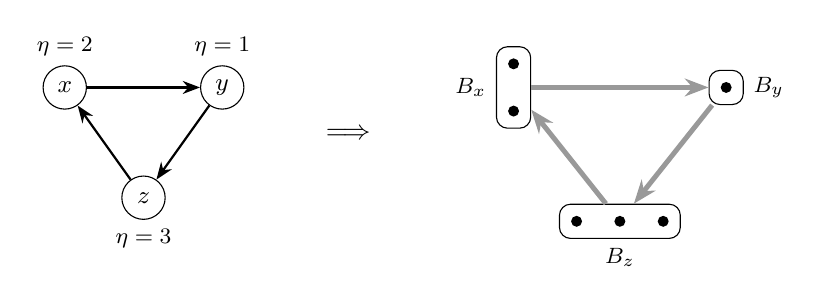
\begin{tikzpicture}
 \begin{scope}
  \node[vtx,label={[font=\footnotesize]above:$\eta=2$}] (x) at (0,0) {$x$};
  \node[vtx,label={[font=\footnotesize]above:$\eta=1$}] (y) at (2,0) {$y$};
  \node[vtx,label={[font=\footnotesize]below:$\eta=3$}] (z) at (1,-1.4) {$z$};
  \draw[arc] (x)--(y); \draw[arc] (y)--(z); \draw[arc] (z)--(x);
 \end{scope}
 \node at (3.6,-0.6) {$\Longrightarrow$};
 \begin{scope}[xshift=6cm]
  \node[dot] (x1) at (-0.3,0.3) {}; \node[dot] (x2) at (-0.3,-0.3) {};
  \node[dot] (y1) at (2.4,0) {};
  \node[dot] (z1) at (0.5,-1.7) {}; \node[dot] (z2) at (1.05,-1.7) {}; \node[dot] (z3) at (1.6,-1.7) {};
  \node[draw,rounded corners,fit=(x1)(x2),inner sep=4pt,label={[font=\footnotesize]left:$B_x$}] (Bx) {};
  \node[draw,rounded corners,fit=(y1),inner sep=4pt,label={[font=\footnotesize]right:$B_y$}] (By) {};
  \node[draw,rounded corners,fit=(z1)(z3),inner sep=4pt,label={[font=\footnotesize]below:$B_z$}] (Bz) {};
  \draw[-{Stealth[length=3mm]},line width=1.8pt,black!40] (Bx)--(By);
  \draw[-{Stealth[length=3mm]},line width=1.8pt,black!40] (By)--(Bz);
  \draw[-{Stealth[length=3mm]},line width=1.8pt,black!40] (Bz)--(Bx);
 \end{scope}
\end{tikzpicture}
\caption{Reducing integer weights to \cref{thm:main}: vertex $x$ of weight
$k_x$ becomes an independent set $B_x$ of size $k_x$, and each arc becomes
a complete bipartite set of arcs. Out-neighborhoods at distance one and
two are blown up by exactly the weights.}
\label{fig:weights}
\end{figure}

\begin{proof}[Proof of \textup{(ii)}]
Let $M$ be the $V\times V$ matrix with $M_{v,s}=1$ if $s\in\Ntwo(v)$, $M_{v,s}=-1$ if
$s\in\Nout(v)$, and $0$ otherwise. So $(M\eta)_v=\eta(\Ntwo(v))-\eta(\Nout(v))$. We use
the following form of Farkas' lemma (Ville's theorem): either there is
$\eta\ge0$, $\eta\ne0$, with $M\eta\ge0$, or there is $\xi\ge0$ with $M^\T\xi<0$ in every
coordinate.

\emph{Derivation from Farkas' lemma.} The system $\xi\ge0$, $M^\T\xi\le-\mathbf 1$ is
infeasible exactly when there is $\eta\ge0$ with $M\eta\ge0$ and
$\eta^\T(-\mathbf 1)<0$, i.e.\ $\eta\ne0$. Rescaling shows that $M^\T\xi<0$ is
solvable if and only if $M^\T\xi\le-\mathbf1$ is.

Now let $\overleftarrow D$ be $D$ with all arcs reversed. Then
$s\in N^+_{k,\overleftarrow D}(v)$ if and only if $v\in N^+_{k,D}(s)$ for
$k=1,2$, so the matrix of $\overleftarrow D$ is $M^\T$. The second alternative
would say $\xi(\Ntwo(v))<\xi(\Nout(v))$ for every vertex $v$ of $\overleftarrow D$,
contradicting (i) for $\overleftarrow D$ with weighting $\xi$. So the first
alternative holds, and normalizing $\eta$ gives (ii).
\end{proof}

\begin{proof}[Proof of \textup{(iii)}]
Seacrest~\cite[Proposition~2]{Seacrest2015} proved that the arc-weighted
statement for all oriented graphs is equivalent to \cref{thm:main}.
\end{proof}

Setting $w(us)=\eta(s)$ for every arc $us$ turns (iii) into (i): if $s\in\Nout(v)$,
all differences $w(us)-w(vs)$ vanish, and if $s\in\Ntwo(v)$, then $w(vs)=0$ and
$\beta^w_v(s)=\eta(s)$. So (iii) is the most general of the three forms.

\subsection{Directed triangles}\label{sec:triangles}

In an oriented graph without directed triangles, the second
out-neighborhood of $v$ avoids both the in- and out-neighbors of $v$. So
\cref{thm:main} produces a vertex with many non-neighbors.

\begin{corollary}[Non-neighbors and directed triangles]\label{cor:triangles}
Let $D$ be a nonempty oriented graph on $n$ vertices. Write
$N^-_1(v)=\{u:u\to v\}$, $d^\pm(v)=\abs{N^\pm_1(v)}$, $\delta^\pm(D)=\min_xd^\pm(x)$, and let
\[
 \overline N(v)=V(D)\setminus\bigl(\{v\}\cup N^+_1(v)\cup N^-_1(v)\bigr)
\]
be the set of non-neighbors of $v$.
\begin{enumerate}[label=\textup{(\roman*)}]
\item If $D$ has no directed triangle, then some vertex $v$ satisfies
$d^+(v)\le\abs{\overline N(v)}$, and hence $n-1\ge2d^+(v)+d^-(v)$.
\item If $\delta^+(D)\ge n/3$ and $\delta^-(D)\ge n/3$, then $D$ contains a directed triangle.
\item If $D$ is $r$-regular ($d^+=d^-=r\ge1$ everywhere) and its shortest
directed cycle has length exactly $4$, then $n\ge3r+1$.
\end{enumerate}
\end{corollary}

Statement (i) is the oriented case of a non-neighbor conjecture of
Thomass\'e recorded in~\cite[Conjecture~6.12]{Sullivan2006}. Statement
(iii) is the girth-four case of the Behzad--Chartrand--Wall
conjecture~\cite{BehzadChartrandWall1970}, see~\cite[Section~4]{Sullivan2006}.

\begin{figure}[ht]
\centering
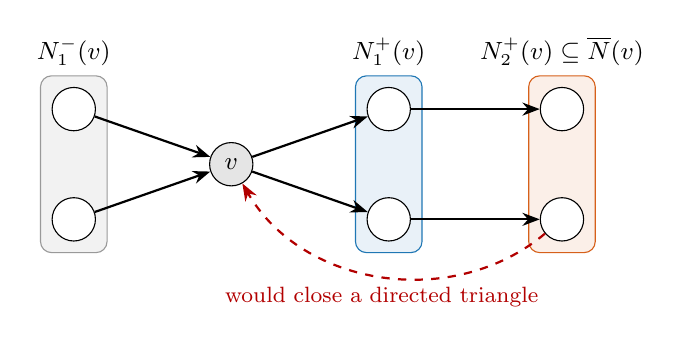
\begin{tikzpicture}
 \node[vtx,fill=black!10] (v) at (0,0) {$v$};
 \node[vtx] (o1) at (2,0.7) {}; \node[vtx] (o2) at (2,-0.7) {};
 \node[vtx] (i1) at (-2,0.7) {}; \node[vtx] (i2) at (-2,-0.7) {};
 \node[vtx] (w1) at (4.2,0.7) {}; \node[vtx] (w2) at (4.2,-0.7) {};
 \draw[arc] (v)--(o1); \draw[arc] (v)--(o2);
 \draw[arc] (i1)--(v); \draw[arc] (i2)--(v);
 \draw[arc] (o1)--(w1); \draw[arc] (o2)--(w2);
 \draw[arc,red!70!black,dashed] (w2) to[out=-140,in=-60] node[below,font=\footnotesize] {would close a directed triangle} (v);
 \begin{scope}[on background layer]
  \node[draw=famL,fill=famL!10,rounded corners,fit=(o1)(o2),inner sep=4pt,label={[font=\small]above:$N^+_1(v)$}] {};
  \node[draw=black!40,fill=black!5,rounded corners,fit=(i1)(i2),inner sep=4pt,label={[font=\small]above:$N^-_1(v)$}] {};
  \node[draw=famR,fill=famR!10,rounded corners,fit=(w1)(w2),inner sep=4pt,label={[font=\small,align=center]above:$\Ntwo(v)\subseteq\overline N(v)$}] {};
 \end{scope}
\end{tikzpicture}
\caption{Without directed triangles, a vertex at distance two from $v$ cannot be
an in-neighbor of $v$. So $\Ntwo(v)$ consists of non-neighbors.}
\label{fig:triangles}
\end{figure}

\begin{proof}
(i) Let $w\in\Ntwo(v)$ via $v\to u\to w$. By definition $w\ne v$ and $w\notin\Nout(v)$. If
$w\in N^-_1(v)$, then $v\to u\to w\to v$ would be a directed triangle. So
$\Ntwo(v)\subseteq\overline N(v)$, and a Seymour vertex $v$ (\cref{thm:main}) has
$d^+(v)\le\abs{\Ntwo(v)}\le\abs{\overline N(v)}$. As $D$ is oriented, $N^+_1(v)$ and $N^-_1(v)$
are disjoint, so $n-1=d^+(v)+d^-(v)+\abs{\overline N(v)}\ge2d^+(v)+d^-(v)$.

(ii) Without a directed triangle, (i) gives $n-1\ge2\delta^+(D)+\delta^-(D)\ge n$, which is
impossible. (Since degrees are integers, the hypothesis means
$\delta^\pm\ge\lceil n/3\rceil$, which includes the case $3\mid n$.)

(iii) Girth four excludes directed triangles, and (i) gives $n-1\ge3r$.
\end{proof}

\appendix
\section{Dictionary and remarks on the original preprint}\label{app:dictionary}

\paragraph{Correspondence of results.}
\begin{center}\small
\begin{tabular}{@{}ll@{}}
\toprule
This document & Original preprint\\
\midrule
\cref{thm:main} & Theorem 1.1\\
\cref{lem:strong,lem:subset-deficit} & Lemma 2.2\\
\cref{lem:internal,lem:blowup} & Lemma 2.3\\
\cref{prop:reduction} & Proposition 2.1\\
\cref{lem:pruning} & Lemma 3.1\\
\cref{lem:kernel} & Lemma 3.2\\
\cref{prop:matching-bound} & the matching bound inside the proof of Lemma 3.1\\
\cref{prop:no-concave} & Proposition 4.1\\
\cref{cor:weighted,cor:triangles} & Corollaries 5.1 and 6.1\\
\bottomrule
\end{tabular}
\end{center}

\paragraph{Changes of notation.}
To avoid clashes we write $\mu=\abs P+\abs Q$ (the original uses $M$, which
we reserve for matchings $\Mm$ and the matrix of \cref{cor:weighted});
$\unc(P,Q)$ for the number $d$ of uncovered points; $\Phi^{p,i}$ for the
matrix $D^{p,i}$ (since $D$ denotes a graph); $\overline N(v)$ for the
non-neighbors $Z(v)$ (since $Z$ denotes conflict points); and
$\mathrm{Arc}(D)$ for the arc set $A(D)$ (since $A$ is a matrix). We added the
names $\val$, ``admissible'', $\Gamma_L$, $\Gamma_N$, $R_1$, $\kappa$.
Otherwise the notation is that of the original.

\paragraph{Remarks.}
We checked every step of the original and found \textbf{no mathematical
error}. The following points are only implicit there, and we have made them
explicit.
\begin{enumerate}[leftmargin=*]
\item Lemma~2.2 in the original states strong connectivity together with
the subset deficit. Strong connectivity is exactly what is needed for
$E=F(S)\setminus S\ne\varnothing$, and it is the reason why the number of
vertices is minimized before the number of arcs (\cref{lem:strong}).
\item The proof of the blow-up lemma uses only the integrality of the
subset deficit and the inequality~\eqref{eq:blowup-master}. The latter holds
in \emph{every} blow-up of every oriented graph. We isolated it, together
with its unblown-up version~\eqref{eq:error-term}, to explain why the
blow-up is used (\cref{rem:error-term}).
\item In the pruning lemma, the bound~\eqref{eq:pruning-bound} is not a
bound on the minimum number of deletions (\cref{ex:K22}). This is easy to
misread, so we added an explicit example.
\item In the matching bound, the step $\rank(NL)\ge\ell+t-\abs Z$ is Sylvester's
rank inequality, and the choice of a maximum matching with the fewest
conflict edges is used only to make $\alpha,\beta$ maximum in their
subgraphs (\cref{cl:alpha-max}).
\item Seacrest's equivalences~\cite{Seacrest2015} are needed only for the
arc-weighted form. The vertex-weighted forms follow from \cref{thm:main}
by the short argument in \cref{sec:weighted}.
\item The bibliographic and historical statements in the introduction are
taken from the original preprint and were not independently verified.
\end{enumerate}

\section{Computer checks and formalization}\label{app:checks}

\sloppy
\paragraph{Randomized tests.}
The folder \texttt{checks/} contains three dependency-free Python scripts.
\texttt{check\_pruning.py} builds, for thousands of random relations on
$2$--$5$ points and random families $\Rf,\Cf$, the graph $\Gamma$. It verifies
$\nu(\Gamma)\le\abs Z+\abs H$ (\cref{prop:matching-bound}), checks that the
K\H{o}nig cover produces a pruning with \ref{P1}--\ref{P3}, and confirms by
exhaustive search that a valid pruning exists. The bound is attained in
roughly a quarter of the instances with conflicts, so it is sharp.
\texttt{check\_reduction.py} verifies the unconditional
inequality~\eqref{eq:blowup-master} for random blow-ups, the increment
identity~\eqref{eq:g-increment}, and \cref{cl:diag-free,cl:H-uncovered} for
random admissible pairs (these do not need concavity).
\texttt{check\_small\_graphs.py} runs through \emph{all} labelled oriented
graphs on at most $6$ vertices ($14{,}348{,}907$ on six vertices; about two
minutes). It confirms \cref{thm:main} for each of them and confirms
\cref{prop:no-concave} directly: none of the $5{,}545{,}708$ graphs on six
vertices with positive indegrees is strictly concave. All tests pass. They are sanity checks, not proofs.

\paragraph{Lean formalization.}
The folder \texttt{SeymourLean/} is a Lean~4 project using Mathlib (tag
\texttt{v4.35.0}) that formalizes the \emph{entire} proof of
\cref{thm:main}. The main formal statement is
\begin{center}\small
\texttt{theorem Seymour.seymour\_second\_neighbourhood (V : Type) [Fintype V]
[DecidableEq V] [Nonempty V] (adj : V $\to$ V $\to$ Prop) [DecidableRel adj]
(hor : IsOriented adj) : $\exists$ v, (N1 adj v).card $\le$ (N2 adj v).card}
\end{center}
where \texttt{IsOriented} means irreflexive and asymmetric, \texttt{N1 v} is
the set of out-neighbors, and \texttt{N2 v} is the set of $w\ne v$ with
$v\not\to w$ and $v\to u\to w$ for some $u$. \texttt{lake build} checks it with
no \texttt{sorry}, and \texttt{\#print axioms} reports only Lean's standard
axioms \texttt{propext}, \texttt{Classical.choice} and \texttt{Quot.sound}.
The file \texttt{SeymourLean/build.log} records a full build together with
the output of \texttt{lake env lean CheckAxioms.lean}, so this can be checked
without rebuilding. The files follow the paper:
\begin{itemize}
\item \texttt{Reduction.lean}: minimal counterexample, \cref{lem:strong} and
\cref{lem:subset-deficit};
\item \texttt{BlowUp.lean}: \cref{lem:blowup};
\item \texttt{Contradiction.lean}: \cref{prop:no-concave} from the pruning lemma;
\item \texttt{Konig.lean}, \texttt{Gamma.lean}: K\H{o}nig's theorem (derived from
Mathlib's Hall theorem) and \cref{cl:cover-to-pruning};
\item \texttt{LinAlg.lean}, \texttt{Generic.lean}, \texttt{MatchingCore.lean},
\texttt{MatchingBound.lean}: Sylvester's inequality, the kernel lemma
(\cref{lem:kernel}), $NL=AB$, \cref{cl:conflict-kernel},
\cref{prop:matching-bound}, and \cref{lem:pruning};
\item \texttt{Final.lean}: the unconditional theorem;
\item \texttt{Insights.lean}: the remarks of the insights pass, see below.
\end{itemize}
The remarks added in \cref{sec:story,sec:ledger,sec:pruning,sec:contradiction}
are formalized in \texttt{Insights.lean}: \texttt{F1\_F2\_comm} ($\Ff\Fs=\Fs\Ff$)
and \texttt{kronecker\_comm} (\cref{rem:kronecker});
\texttt{diag\_compatible\_iff\_oriented} and
\texttt{exists\_admissible\_iff\_oriented} (\cref{lem:admissible-iff-oriented});
\texttt{conflict\_swap}, \texttt{Zset\_swap}, \texttt{Hset\_swap}
(\cref{rem:reversal}); \texttt{gain\_identity} (the exact form of
\cref{cl:gain}) and \texttt{moved\_identity} (\cref{rem:move-repair});
and \texttt{step\_ledger}, \texttt{step\_value}: for an arbitrary relation
and any admissible pair, pruning the complements gives an admissible pair of
value at least $\val(P,Q)-\sum\kappa$ (\cref{rem:algorithm}), with no
concavity assumed. Not formalized: the Dulmage--Mendelsohn reading of the
kernel lemma (\cref{rem:DM}), the computer observations of
\cref{rem:combinatorial}, and the running-time statement of
\cref{rem:algorithm}. \texttt{CheckAxioms.lean} prints the axioms of
these theorems as well.
A few steps are argued differently in Lean. Generic coefficients are taken
as the variables themselves in the fraction field of a polynomial ring
rather than as a real point. Only $\rank L\ge\ell$ is used, obtained from
Hall's theorem and an exchange argument, instead of the full statement
$\rank L=\nu(\Gamma_L)$. The rank count goes through the three-term complex of \cref{sec:rank}
(\texttt{ComplexCount.lean}: \texttt{complex\_count} is the counting of
\cref{cl:kerA,cl:rank-inequality}, and \texttt{dimension\_count} is
\cref{cl:rank-inequality} for the matrices of the paper); the earlier
version of the project used Sylvester's inequality twice instead. Strong connectivity is replaced by ``every nonempty
proper set has an arc leaving it''. The formalization found no mathematical
error in the paper. It also shows that the pruning lemma holds for an
arbitrary relation and that orientation is used exactly at the places listed
in \cref{rem:hypotheses}.



\bibliographystyle{plain}
\bibliography{references}
\end{document}
